
% Citation fixes: ref475512852976725 -> mobilefish_lora_tutorial_2016; ref528894793712157 -> pajooh2022experimentalperformanceanalysis; suarez_albela_2018 -> suarez_albela_2018; ref466387264872117 -> klaassen_2025; ref76853680998234 -> forchag_evaluation_2024; ref982941445060204 -> bodkhe2022blockchainforprecision; ref510439910314487 -> hyperledger_walmart_2020; ref947524953303383 -> wef_gdpr_2020; ref167328542643761 -> gsci_blockchain_supplychain_2022; ref770016859057512 -> batchit_2024; ref476767734630149 -> melo2025comprehensive; ref995547205066438 -> klaassen_2025

\documentclass[12pt,onecolumn]{IEEEtran} % single-column, 12pt

% --- Essential packages ---
\usepackage{lscape}  
\usepackage[utf8]{inputenc}
\usepackage{pdflscape}
\usepackage[T1]{fontenc}
\usepackage[utf8]{inputenc}
\usepackage{lmodern} % Better font support
\usepackage{amsmath,amssymb,amsfonts}
\usepackage{algorithmic}
\usepackage{graphicx}
\usepackage{xcolor}
\usepackage{textcomp}
\usepackage{microtype}
\usepackage{siunitx} % Added for proper unit formatting
\usepackage{enumitem}
\usepackage{tikz}
\usetikzlibrary{arrows.meta,positioning,fit}

\usepackage{pgfplots,pgfplotstable}
\pgfplotsset{compat=1.17} % or newer if your TeX supports it
\usepackage{siunitx}
\sisetup{detect-all}

\usepackage{tabularx,booktabs}   % for the table
\usepackage{tikz}                % for the schematic
\usetikzlibrary{positioning,fit,calc} % minimal, robust set

\usepackage{pgfplots,pgfplotstable}
\pgfplotsset{compat=1.18}

% --- Page layout ---
\usepackage[margin=1in]{geometry}

% --- TikZ + helpers (safe for cloud shapes) ---
\usepackage{tikz}
\usetikzlibrary{arrows.meta,positioning,fit,calc,backgrounds,shapes.symbols,shapes.multipart}
\usepackage{adjustbox} % to auto-fit figure to text width

% --- Plots with error bars ---
\usepackage{pgfplots,pgfplotstable}
\pgfplotsset{compat=1.17} % adjust if your TeX is newer
\usepgfplotslibrary{groupplots}
\usepackage{siunitx}
\sisetup{detect-all}

% --- Font & spacing ---
\usepackage{newtxtext,newtxmath}
\usepackage{setspace}
\AtBeginDocument{\setstretch{1.5}}  % 1.5 line spacing
\usepackage{footmisc}
\setlength{\footnotesep}{1.5\baselineskip} % Adjust footnote spacing

% --- Table packages ---
\usepackage{array}
\usepackage{tabularx}
\usepackage{booktabs} % you already use \toprule/\midrule/\bottomrule
\usepackage{adjustbox}
\usepackage{ragged2e}
\usepackage{float}

% Custom column types
\newcolumntype{L}[1]{>{\raggedright\arraybackslash}p{#1}} % fixed-width, ragged-right
\newcolumntype{Y}{>{\raggedright\arraybackslash}X}        % flexible-width, ragged-right
\newcolumntype{P}[1]{>{\RaggedRight\arraybackslash}p{#1}} % fixed-width ragged-right column
\newcommand{\fitToPage}[1]{\begin{adjustbox}{max width=\textwidth}#1\end{adjustbox}}

% Table formatting
\setlength{\tabcolsep}{6pt}  % Adjusts column spacing
\renewcommand{\arraystretch}{1.2} % Set to 1.5 if you want table rows also at 1.5

% --- Section formatting ---
\usepackage{titlesec}
\titleformat{\part}[display]
  {\normalfont\bfseries\fontsize{14pt}{16.8pt}\selectfont}  % 14pt, bold
  {\partname~\thepart}{0.5em}{}
\titleformat{\section}
  {\normalfont\bfseries\fontsize{14pt}{16.8pt}\selectfont}
  {\thesection}{1em}{}
\titleformat{\subsection}
  {\normalfont\bfseries\fontsize{12pt}{14pt}\selectfont}
  {\thesubsection}{1em}{}
\titleformat{\subsubsection}
  {\normalfont\itshape\fontsize{12pt}{14pt}\selectfont}
  {\thesubsubsection}{1em}{}

% Section spacing
\titlespacing*{\section}{0pt}{*2}{*1}
\titlespacing*{\subsection}{0pt}{*1.5}{*0.8}
\titlespacing*{\subsubsection}{0pt}{*1.2}{*0.6}


% ------------------ Minimal preamble for CircuitikZ/TikZ figures ------------------
\usepackage[T1]{fontenc}
\usepackage[utf8]{inputenc}

% Graphics + TikZ
\usepackage{graphicx,xcolor}
\usepackage{tikz}
\usetikzlibrary{positioning,arrows.meta,calc} % used by the figures

% Circuit schematics
\usepackage[siunitx,american]{circuitikz} % CircuitikZ with American symbols/voltages

% Units/symbols (for \SI, \si, and \ohm if you keep it)
\usepackage{siunitx}
\sisetup{detect-all,per-mode=symbol}

% Older docs sometimes need this for \ohm in text labels:
\usepackage{textcomp} % provides \ohm (if you prefer \SI{100}{\ohm}, this line is optional)

% (Optional) page layout and captions
\usepackage[margin=1in]{geometry}
\usepackage{caption}
% ------------------------------------------------------------------------------


% --- Numbering format ---
\setcounter{secnumdepth}{3}
\setcounter{tocdepth}{3}

\makeatletter
\renewcommand\thesection{\arabic{section}}
\renewcommand\thesubsection{\thesection.\arabic{subsection}}
\renewcommand\thesubsubsection{\thesubsection.\arabic{subsubsection}}

% For table of contents
\renewcommand{\numberline}[1]{\hb@xt@\@tempdima{#1\hfil}}
\makeatother

% --- Captions ---
\usepackage{caption}
\captionsetup{font={small,stretch=1.5}}  % Captions with 1.5 line spacing and small font size

% --- Hyperlinks & references ---
\usepackage[hyphens]{url}
\Urlmuskip=0mu plus 1mu
\usepackage[hidelinks]{hyperref}
\hypersetup{
    pdftitle={Blockchain-enabled IoT Framework for Smart Agriculture},
    pdfauthor={},
    pdfpagemode=UseOutlines,
}
\usepackage{cite}

% --- Table of Contents formatting with tocloft package ---
\usepackage{tocloft}
\setlength{\cftsecindent}{0em}     % No indent for sections
\setlength{\cftsubsecindent}{1.5em} % Indent for subsections
\setlength{\cftsubsubsecindent}{3em} % Indent for subsubsections
\setlength{\cftsecnumwidth}{2.5em}  % Adjust the number width for sections
\setlength{\cftsubsecnumwidth}{3.5em} % Adjust the number width for subsections
\setlength{\cftsubsubsecnumwidth}{4em} % Adjust the number width for subsubsections
\setlength{\cftbeforesecskip}{1em}   % Space before each section in ToC
\setlength{\cftbeforesubsecskip}{0.5em} % Space before each subsection
\setlength{\cftbeforesubsubsecskip}{0.5em} % Space before each subsubsection

% ---- Title (bold) ----
\title{\textbf{Results and Discussion}}
\author{} % optional
\date{}   % optional

\begin{document}

% ---- Title (bold) ----
\title{\textbf{Results and Discussion}}
\author{} % optional
\date{}   % optional
% --- Table of Contents ---
\tableofcontents
\clearpage
% ---------- Local macros ----------
\newcommand{\CurrentP95L}{\textbf{[SET: e.g., 1.7\,s]}}
\newcommand{\CurrentP99L}{\textbf{[SET: e.g., 2.6\,s]}}
\newcommand{\CurrentTPS}{\textbf{[SET: e.g., 45\,tx/s]}}
\newcommand{\CurrentRel}{\textbf{[SET: e.g., 0.992]}}
\newcommand{\CurrentAvail}{\textbf{[SET: e.g., 0.997]}}
\newcommand{\SLOpL}{\textbf{$p95(L)\!\!<\!2$\,s}}
\newcommand{\SLOpLnn}{\textbf{$p99(L)\!\!<\!3$\,s}}
\newcommand{\SLOR}{\textbf{$R\!\ge\!0.99$}}
\newcommand{\SLOA}{\textbf{$A\!\ge\!0.995$}}
% -----------------------------------------------------------------------------------------------
% ===================== FIGURE/TABLE LABEL ALIASES (EDIT THESE ONLY IF NEEDED) =====================
% Map these to your existing labels so references in text & tables match exactly.
\providecommand{\figPipelineLatencyCDF}{fig:pipeline-latency-cdf} % e.g., set to fig:fig1 if that's your latency CDF
\providecommand{\figBundleLatencyBox}{fig:bundle-latency-box}     % e.g., set to fig:fig2
\providecommand{\figReliabilityAvailability}{fig:reliability-availability}
\providecommand{\figBacklogTrend}{fig:backlog-trend}
\providecommand{\figThroughputVsEnergy}{fig:throughput-vs-energy}
\providecommand{\tabLedgerGrowth}{tab:ledger-growth}
\providecommand{\tabWireBytes}{tab:wire-bytes}
\providecommand{\tabChurnOutcomes}{tab:churn-outcomes}

% ===================== CHAPTER START =====================
\section{Introduction}
\label{sec:introduction}

This chapter presents the experimental evaluation of a blockchain-enabled Internet of Things (IoT) framework for smart agriculture. We analyze performance, scalability, reliability, security, and Quality of Service (QoS) under field-relevant conditions. A central question is whether a \emph{Chinese Remainder Theorem (CRT)-based parallel transaction model} can narrow the throughput–latency gap relative to lightweight or hybrid designs while preserving immutability and traceability.

\paragraph{System Goals.} The system is designed to:
\begin{enumerate}
    \item Provide verifiable, near-real-time sensing for irrigation control and crop health monitoring.
    \item Utilize compact, energy-aware transaction payloads via CRT residues for data compression.
    \item Implement a hierarchical validation architecture from sensors to gateways and finally to a permissioned ledger (Hyperledger Fabric).
    \item Ensure long-term auditability through daily anchoring of data summaries to a blockchain.
\end{enumerate}

% --------------------------------------------------------------------------
\subsection{Research Questions, Service Level Objectives, and Hypotheses}
\label{sec:rqs-slos}

\textbf{Research Questions (RQs).}
\begin{enumerate}
    \item[\textbf{RQ1:}] Can CRT-based partitioning of sensor payloads and transaction fields reduce on-chain payload size and batching delay sufficiently to maintain the \textbf{95th-percentile (p95) latency target} (95\% of operations complete within 2\,s) and the \textbf{99th-percentile (p99) latency target} (99\% complete within 3\,s) under realistic field conditions?
    \item[\textbf{RQ2:}] Does a hierarchical, edge-assisted consensus model (Fabric ordering at the core with lightweight consensus at the edge) sustain the \textbf{reliability SLO ($R \geq 0.99$)} and the \textbf{availability SLO ($A \geq 0.995$)} when nodes experience intermittent connectivity?
    \item[\textbf{RQ3:}] What is the throughput–energy trade-off when combining CRT residue compression with daily Merkle anchoring to a public chain, compared with a fully on-chain storage approach?
\end{enumerate}

\textbf{Service Level Objectives (SLOs).}
Unless stated otherwise, targets apply to the \emph{write} path:
\begin{itemize}
    \item \textbf{p95 latency target}: 95\% of operations complete within 2\,s.
    \item \textbf{p99 latency target}: 99\% of operations complete within 3\,s.
    \item \textbf{Reliability ($R$)}: Probability a write commits under its deadline, with $R \geq 0.99$.
    \item \textbf{Availability ($A$)}: Fraction of time intervals during which the system meets its SLOs, with $A \geq 0.995$.
    \item \textbf{Steady-state throughput}: Sufficient to absorb burst uploads (e.g., 120–150 sensor readings/s/ha) within a sub-5\,s window.
\end{itemize}

\textbf{Hypotheses.}
\begin{enumerate}[leftmargin=*, itemsep=0.4em]
  \item \textbf{H1 (Latency):} Sharding numeric data fields into CRT residues and reconstructing off-chain reduces per-transaction byte size and queuing delays, yielding lower batch dwell times and decreased \textbf{p95}/\textbf{p99} latency compared with plain encoding at the same transactions-per-second (TPS) rate.
  \item \textbf{H2 (Reliability/Availability):} Edge-level aggregation with periodic anchoring decouples local writes from the public anchoring schedule, maintaining \textbf{reliability} ($R$) and \textbf{availability} ($A$) at or above target thresholds under link churn and intermittent connectivity.
  \item \textbf{H3 (Throughput/Energy):} CRT compression combined with daily Merkle anchoring reduces load on on-chain storage and the ordering service, enabling higher throughput (tx/s) for equivalent CPU and network budgets; lightweight or domain-specific BFT variants further reduce message complexity and energy per committed transaction~\cite{haque2024scalable,coinspaid2023dag}.
\end{enumerate}

% ===================== EXPERIMENT DESIGN (FULLY FACTORED) =====================
\subsection{Experiment Design, Factors, and Success Criteria}
\label{sec:exp-design}

\paragraph{Assumptions and Testbed.}
Experiments run on the five-tier pipeline: Tier~1 ESP32 leaves; Tier~2 Raspberry Pi gateways (Ingress/Bundler/Scheduler); Tier~3 Pi$\leftrightarrow$Pi mesh (BATMAN-adv L2 + WireGuard); Tier~4 Hyperledger Fabric (Raft orderers + peers on Pis); Tier~5 observability (Prometheus/Grafana/Alertmanager).
Unless stated, payload budget at the leaf is 100\,B; CRT is enabled \emph{only} when the computed packet size exceeds this budget. Fabric \texttt{BatchTimeout} $\in \{2,3,5\}$\,s; event coalescing $\in[60,120]$\,s; periodic window $W\in\{30,60,120\}$\,min. Orderer count is $\{1,3\}$ (odd quorum when $\geq 20$ gateways). All TLS links are enabled.

\paragraph{Workloads (field-relevant).}
We use two workload classes:
\begin{enumerate}[leftmargin=*, itemsep=0.25em]
  \item \textbf{Periodic sensing (windowed)}: $S\in\{5,8,12\}$ sensors/node; one reading every $\{30,60,120\}$\,s; window sizes $W$ above. Each reading emits statistics $\{\text{min},\text{avg},\text{max},\text{std},\text{count}\}$.
  \item \textbf{Event-driven bursts}: threshold breaches generate immediate EventBundles; per-node event rate $\lambda_e\in\{0,1/10\text{\,min},1/5\text{\,min}\}$; rate-limited to $\leq6$/h with coalescing $\in[60,120]$\,s.
\end{enumerate}
Scale-out: gateways $N_{\text{pi}}\in\{2,20,100\}$; leaves per gateway $L\in\{5,10,25\}$.

\paragraph{Network and Mesh (Tier~3).}
Hop count $H\in\{0,1,2,3,5\}$; per-hop latency target ``few ms'', measured as \texttt{per\_hop\_latency\_ms}. Controlled churn: packet loss $\in\{0\%,3\%,8\%\}$; jitter $\in\{5,10,15\}$\,ms; outage intervals with on/off durations $(t_{\text{down}},t_{\text{up}})\in\{(10\text{\,s},5\text{\,min}),(60\text{\,s},5\text{\,min}),(120\text{\,s},5\text{\,min})\}$. ETX thresholds trigger reroute. Minimum neighbors $\geq 2$ unless testing failure drills.

\paragraph{CRT Moduli and Byte Budget (Tiers~1--2).}
Payload accounting uses concrete field sizes (IDs/timestamps/flags/signature + $S\times5$ stats). When budget $>100$\,B:
\begin{itemize}[leftmargin=*, itemsep=0.1em]
  \item \textbf{Moduli bands} (\emph{pairwise coprime}): 
    \begin{itemize}[leftmargin=1.25em]
      \item memory $<32$\,KiB $\rightarrow$ $[97,101]$ (2 residues, $\approx 2$\,B/value)
      \item $32$--$64$\,KiB $\rightarrow$ $[97,101,103]$ (3 residues, $\approx 3$\,B/value)
      \item $>64$\,KiB $\rightarrow$ $[97,101,103,107]$ (4 residues, $\approx 4$\,B/value)
    \end{itemize}
  \item \textbf{Selection rule}: choose smallest band whose product covers the integer range of the encoded field group; reconstruct with Garner; verify $x<\prod m_i$ before Merkle hashing.
\end{itemize}

\paragraph{Fabric Policy (Tier~4).}
\texttt{BatchTimeout}$\in\{2,3,5\}$\,s; \texttt{MaxMessageCount}$\in\{10,25,50\}$; \texttt{PreferredMaxBytes}$\in[1,2]$\,MB; \texttt{AbsoluteMaxBytes}$=10$\,MB. Orderers $\in\{1,3\}$; peers on Pis; CouchDB with JSON indexes on \texttt{device\_id}, \texttt{window\_id}, \texttt{ts}. Endorsement policy minimal for write path (bundler client identity). 

\paragraph{Energy Measurement (Throughput/Energy).}
Energy/tx (J/tx) measured at Tier~2 gateway + mesh radio path using inline power measurement (or per-node energy counters when present). Sampling at 1\,Hz; integrate over experiment window; divide by committed tx count. CPU load and network IO gathered from OS counters.

\paragraph{Metrics and Instrumentation.}
\begin{itemize}[leftmargin=*, itemsep=0.1em]
  \item \textbf{Latency}: submit$\to$commit histogram (\texttt{submit\_commit\_seconds}) with p50/p95/p99; Tier~2 \texttt{bundle\_latency\_seconds}.
  \item \textbf{Reliability/Availability}: $R$ = Pr(commit under deadline); $A$ = fraction of time intervals where SLOs are met; missed-window count; backlog trend \texttt{t2:store\_backlog\_files}.
  \item \textbf{Throughput}: committed tx/s, block cuts/min, on-chain bytes/day, orderer CPU.
  \item \textbf{Network/Mesh}: \texttt{per\_hop\_latency\_ms}, \texttt{mesh\_neighbors}, retries/ETX/jitter, path changes.
  \item \textbf{Bytes on wire}: payload bytes/reading (leaf$\to$Pi), bundle size, block size.
  \item \textbf{Energy}: J/tx for client path (Tier~2 + mesh radio).
\end{itemize}

\paragraph{Experimental Controls and Randomization.}
Each scenario uses: 10\,min warm-up; 30--60\,min steady-state; 5\,min cool-down. Three independent repetitions with different random seeds (event times, jitter/loss). Churn profiles applied via traffic shaper at gateway uplink. Only one factor changes per sweep unless performing 2D grids (marked explicitly).

\paragraph{Statistical Treatment.}
Report medians and 95\% CIs via bootstrap (10k resamples) for latency percentiles and J/tx. Use Cliff’s delta for effect size on pairwise comparisons (CRT-on vs CRT-off; edge-assisted vs direct). Success/failure judged per SLO thresholds or relative deltas (H3).

% ----------------------------- RQs + Hypotheses (Concise) --------------------
\paragraph{Research Questions (RQs).}
\begin{enumerate}
  \item[\textbf{RQ1}] When CRT is enabled only on budget overflow, does end-to-end write latency meet the p95/p99 SLOs under field-relevant workloads and mesh conditions?
  \item[\textbf{RQ2}] Under intermittent connectivity, does edge-assisted design (local writes + store\&forward + periodic anchoring) sustain the reliability and availability SLOs better than a direct-to-ledger baseline?
  \item[\textbf{RQ3}] For equivalent auditability (Merkle proofs vs full on-chain), does CRT + daily anchoring improve the throughput--energy profile relative to fully on-chain storage?
\end{enumerate}

\paragraph{Hypotheses (falsifiable).}
\begin{enumerate}[leftmargin=*, itemsep=0.25em]
  \item \textbf{H1 (Latency effectiveness of budgeted CRT).} 
  Given: budget 100\,B at Tier~1; CRT triggers only when computed packet size exceeds budget; \texttt{BatchTimeout}$\in\{2,3,5\}$\,s; $H\in\{0,1,2,3,5\}$; windows $W\in\{30,60,120\}$\,min; loss$\in\{0\%,3\%,8\%\}$.\\
  \emph{Claim:} Versus plain encoding at matched TPS and topology, budgeted CRT attains p95$\leq$2\,s and p99$\leq$3\,s submit$\to$commit and reduces median Tier~2 batch dwell time by $\geq$20\%.\\
  \emph{Primary metrics:} submit$\to$commit p50/p95/p99; bundle latency; wire bytes/reading.\\
  \emph{Controlled:} $S,L,H,W$, coalescing, \texttt{BatchTimeout}, moduli band.

  \item \textbf{H2 (Resilience under churn).}
  Given: controlled on/off outages and jitter/loss profiles as above; orderers $\in\{1,3\}$.\\
  \emph{Claim:} Edge-assisted pipeline maintains $R\geq0.99$ and $A\geq0.995$ over 24\,h and exhibits non-increasing backlog; a direct-to-ledger baseline violates at least one of these SLOs under identical churn.\\
  \emph{Primary metrics:} $R$, $A$, backlog trend, missed-window count; p99 submit$\to$commit tails.\\
  \emph{Controlled:} outage cadence/duration, orderers, \texttt{BatchTimeout}, neighbors.

  \item \textbf{H3 (Throughput--energy trade-off).}
  Given: same hardware/topology; daily anchoring; identical security policies.\\
  \emph{Claim:} Relative to fully on-chain storage, CRT + daily anchoring achieves either (a) $\geq25\%$ higher tx/s at the same J/tx, or (b) $\geq20\%$ lower J/tx at the same tx/s, while preserving auditability via Merkle proofs.\\
  \emph{Primary metrics:} tx/s, J/tx, orderer CPU, on-chain bytes/day.\\
  \emph{Controlled:} bundle size, anchoring cadence, moduli band, $H$.
\end{enumerate}

% ----------------------------- Factor Grid Table -----------------------------
\begin{table}[htbp]
  \centering
  \caption{Factor grid for experiment sweeps (ranges/levels per tier).}
  \label{tab:factor-grid}
  \begin{tabular}{p{3.2cm} p{10.8cm}}
    \toprule
    \textbf{Factor} & \textbf{Levels / Range} \\
    \midrule
    Sensors per leaf ($S$) & $\{5,8,12\}$; reading period $\{30,60,120\}$\,s \\
    Window length ($W$) & $\{30,60,120\}$\,min (periodic); events immediate \\
    Leaves per gateway ($L$) & $\{5,10,25\}$ \\
    Gateways ($N_{\text{pi}}$) & $\{2,20,100\}$ \\
    Mesh hops ($H$) & $\{0,1,2,3,5\}$; min neighbors $\geq 2$ \\
    Loss / jitter & loss $\{0\%,3\%,8\%\}$; jitter $\{5,10,15\}$\,ms \\
    Outages & $(t_{\text{down}},t_{\text{up}})\in\{(10\text{\,s},5\text{\,min}),(60\text{\,s},5\text{\,min}),(120\text{\,s},5\text{\,min})\}$ \\
    CRT moduli band & $[97,101]$; $[97,101,103]$; $[97,101,103,107]$ (budget-triggered) \\
    Payload budget & 100\,B (leaf) \\
    Coalescing / rate limit & coalesce $[60,120]$\,s; $\leq6$ events/h/node \\
    BatchTimeout & $\{2,3,5\}$\,s; MaxMessageCount $\{10,25,50\}$ \\
    Anchoring cadence & daily (Merkle summaries) \\
    Orderers & $\{1,3\}$; Raft \\
    State DB indexes & JSON indexes on device/window/ts (CouchDB) \\
    \bottomrule
  \end{tabular}
\end{table}

% ----------------------------- Success Criteria Table ------------------------
\begin{table}[htbp]
  \centering
  \caption{Success criteria per RQ/Hypothesis. ``Pass'' requires meeting all listed criteria for that RQ.}
  \label{tab:success-criteria}
  \begin{tabular}{p{2cm} p{9.5cm} p{3.5cm}}
    \toprule
    \textbf{RQ/H} & \textbf{Pass Criteria} & \textbf{Primary Evidence to Provide} \\
    \midrule
    RQ1/H1 &
    p95$\leq$2\,s \& p99$\leq$3\,s (submit$\to$commit) at matched TPS; median bundle dwell $\downarrow\geq$20\% vs.\ plain; wire bytes/reading $\downarrow$ &
    Percentile table (p50/p95/p99), bundle dwell (median/\% change), average wire bytes/reading before vs.\ after \\
    \addlinespace
    RQ2/H2 &
    $R\geq0.99$, $A\geq0.995$ under churn; backlog non-increasing; fewer missed windows vs.\ baseline &
    Reliability/availability summary, backlog statistics (mean/max over window), count of missed-deadline windows \\
    \addlinespace
    RQ3/H3 &
    (a) tx/s $\uparrow\geq25\%$ at same J/tx \emph{or} (b) J/tx $\downarrow\geq20\%$ at same tx/s; on-chain bytes/day $\downarrow$ &
    Throughput vs.\ energy table (tx/s, J/tx), on-chain bytes/day computation, CPU utilisation snapshot \\
    \bottomrule
  \end{tabular}
\end{table}

% --------------- Measurement & Reporting Notes (no figure references) ---------------
\paragraph{Measurement and Reporting Notes.}
\begin{itemize}[leftmargin=*, itemsep=0.15em]
  \item \textbf{Latency distributions:} Report p50/p95/p99 submit$\to$commit for gateway scales $\{2,20,100\}$. Include a small table listing percentiles per scenario; CDF plots are optional.
  \item \textbf{Reliability/Availability under churn:} Provide a table with $R=\Pr\{L\le D_{\max}\}$ (use $D_{\max}=5$\,s unless stated), and $A$ as the fraction of 1\,min intervals meeting the latency and reliability SLOs. Add backlog mean/max over a rolling 30\,min window and the number of missed-deadline windows.
  \item \textbf{Throughput–Energy frontier:} Summarise tx/s and J/tx for CRT{+}anchoring vs.\ full on-chain. Include on-chain bytes/day using
    \[
      \text{ledger\_growth\_day}=\overline{\text{block\_size}}\times\text{blocks/day}.
    \]
    Also list average wire bytes/reading to show compression benefits.
\end{itemize}

% ----------------------------- Threats to Validity (brief) -------------------
\paragraph{Threats to Validity (mitigations).}
Clock skew (mitigate with NTP/GPS-disciplined time); config drift (container pinning); order effects (randomize scenario order); warm-up bias (discard first 10\,min); mesh heterogeneity (repeat with permuted topologies); energy meter accuracy (calibrate, report error band).
\noindent\emph{Context from practice and prior deployments (non-exhaustive):}
\begin{itemize}
    \item[(i)] Private/permissioned food/agri pilots commonly report sub-second app latency and block finalization on the order of a few seconds at small node counts. Our p95 and p99 targets (\textbf{2\,s}, \textbf{3\,s}) are set within those practical bands.
    \item[(ii)] Tailored BFT variants and simplified edge consensus typically reduce end-to-end latency at modest scales. Where ordering capacity is the limiter, byte-size reduction (CRT) plus batching generally increases throughput until peer CPU or state DB I/O becomes the bottleneck.
    \item[(iii)] Hybrid designs minimize on-chain footprint by storing only compact summaries and proofs on-ledger. In this work, we compress payloads at the edge (CRT residues), store summaries on Fabric, and keep raw items available off-ledger via the gateway APIs and exports.
\end{itemize}

\subsection{Metric to Decision Mapping with SLO Alignment}
\label{sec:metric-decision}

The following metrics are mapped to concrete operational actions and evaluated against the SLOs defined earlier. Where possible, they are observable via the repository’s dashboards and scripts (e.g., Flask \texttt{/status}, \texttt{/history}, \texttt{/integrity}; helpers like \texttt{tools/*}, \texttt{channel\_block\_retrieval.py}).

\begin{itemize}
    \item \textbf{Latency, $L$ (end-to-end, p95/p99):} Drives timeliness of irrigation actuation and frost alerts. \textbf{Targets:} \textbf{p95 $\leq$ 2\,s}, \textbf{p99 $\leq$ 3\,s}. \emph{Decision:} If $p95(L)$ meets target, proceed with normal cadence; if $p99(L)>3$\,s, defer non-critical writes to the next batch and reduce bundle sizes until tails recover.
    \item \textbf{Jitter, $J=\sqrt{\mathrm{Var}[D]}$:} High jitter harms closed-loop control (valves/pumps). Aim to keep p95 jitter $<\,$\textbf{0.5\,s} by enforcing maximum bundle dwell and smoothing burst submissions at the gateway. \emph{Decision:} When $J$ spikes, switch to \emph{edge-write with delayed submit} mode.
    \item \textbf{Reliability, $R=\Pr\{D\leq D_{\max}\}$:} Probability a write commits before its deadline. \textbf{SLO: $R \geq 0.99$}. \emph{Decision:} If measured reliability $\CurrentRel<0.99$, lower \emph{BatchTimeout} and bundle size, increase backoff, and enable store\&forward stricter retries at the gateway.
    \item \textbf{Availability, $A$:} Fraction of time intervals meeting all SLOs. \textbf{SLO: $A \geq 0.995$}. \emph{Decision:} If $\CurrentAvail<0.995$, trigger channel-level failover (alternate orderer), and gate readiness on observed block-height advance.
    \item \textbf{Throughput (tx/s):} Must absorb bursts (e.g., tens–hundreds of sensor readings per minute per gateway) with bounded latency. \emph{Decision:} If \CurrentTPS falls below required burst rate, increase block size and parallelize bundle assembly until \textbf{p95} approaches 2\,s or peer CPU saturates.
    \item \textbf{Energy (edge path):} Edge devices and mesh radios should minimize message complexity. \emph{Decision:} If mWh/tx rises during peaks, disable optional heavy crypto on sensors (keep signing minimal) and offload to the gateway; prefer coalesced event bundles.
\end{itemize}

\subsection{Contributions: This Work vs. Prior Art}
\label{sec:contrib-box}

\noindent\fbox{\parbox{\linewidth}{
\textbf{Contributions of this work (implemented in the accompanying repository):}
\begin{enumerate}
    \item \textbf{CRT Residue Compression for Agri-IoT Payloads.} Numeric fields in windowed sensor summaries are partitioned into CRT residues at the leaf/gateway, then reconstructed before Merkle hashing and commit. This reduces per-transaction bytes and bundle dwell. \cite{oh2025foodsafety}.(\texttt{crt\_agri.py}, \texttt{crt\_parallel.py}, \texttt{crt\_utils.py})
    \item \textbf{Hierarchical/Edge-Assisted Consensus.} Gateways ingest and sanitize readings, bundle by window/event, and submit to a Fabric orderer; edge buffering sustains p95/p99 tails under link churn. \cite{haque2024scalable}(\texttt{pi\_gateway.py}, \texttt{edge\_processor.py}, \texttt{hierarchical\_consensus.py}, \texttt{advanced\_consensus.py})
    \item \textbf{Operational Dashboards \& Exports.} A Flask HTTPS UI exposes registration, history, integrity checks, storage, and status; operators can verify on-ledger entries and export CSVs for audit without inflating on-chain storage. \cite{haque2024scalable} (\texttt{flask\_app/app.py}, pages: \texttt{/history}, \texttt{/integrity}, \texttt{/explorer}, \texttt{/storage}, \texttt{/status})
    \item \textbf{End-to-End Testability.} One-click smoke tests and helper scripts bring up a local network, deploy chaincode, emit sample readings, and inspect blocks—supporting reproducible evaluation. \cite{coinspaid2023dag}(\texttt{one\_click\_test.sh}, \texttt{test\_network.sh}, \texttt{channel\_block\_retrieval.py})
\end{enumerate}
}}

\subsection{Alignment with Expected Performance and Trade-offs}
\label{sec:part23-numbers}

Based on small-cluster Fabric setups and the repository’s defaults:
\begin{itemize}
    \item \textbf{Latency:} With tuned \emph{BatchTimeout} and modest block sizes, submit$\to$commit latencies of a few seconds are attainable at low–moderate node counts. Our targets remain \textbf{p95 $\leq$ 2\,s} and \textbf{p99 $\leq$ 3\,s}.
    \item \textbf{Throughput:} Increasing block size and reducing endorsement complexity can raise tx/s until peer CPU or CouchDB indexing dominates. Expected range on Pi-class hardware spans tens to low hundreds of tx/s depending on chaincode complexity and batch policy.
    \item \textbf{Storage Footprint:} Keeping summaries and proofs on-ledger while exporting raw data via the dashboard/API reduces ledger growth versus fully on-chain raw storage.
    \item \textbf{Energy:} Edge-first filtering, coalescing, and residue compression decrease radio airtime and message count, lowering mWh/tx at the client path.\cite{coinspaid2023dag}
\end{itemize}

\subsection{Section Roadmap}
\label{sec:roadmap}

This chapter proceeds as follows: Section~\ref{sec:rqs-slos} states RQs/SLOs and hypotheses. Section~\ref{sec:metric-decision} maps metrics to actions (e.g., irrigation and alerting). Section~\ref{sec:contrib-box} summarizes contributions grounded in the codebase. Section~\ref{sec:part23-numbers} outlines expected ranges and trade-offs. Subsequent sections provide the system design, factor grid, and evaluation plan; mathematical analysis of CRT effects on batch dwell and latency is deferred to later theoretical sections.

\section{System Overview and Experimental Design}
\label{sec:system-overview}

\subsection{Architecture Summary}
\label{subsec:architecture-summary}

ESP32 leaf nodes collect environmental metrics and apply local thresholds. Readings are forwarded over LoRa or HTTP to Raspberry Pi gateways. Gateways verify, de-duplicate, and bundle records, optionally encoding large numeric groups as CRT residues. A Flask HTTPS API (\texttt{flask\_app/app.py}) supports device registration, history lookup, integrity verification, and exports. Bundles are submitted to a local Hyperledger Fabric network where a Go chaincode (\texttt{chaincode/sensor/sensor.go}) records summaries and events. Helper scripts (\texttt{test\_network.sh}, \texttt{one\_click\_test.sh}) start the network and deploy the contract.

\subsubsection{Communication and Data Flow}
\label{subsubsec:communication-data-flow}

\begin{enumerate}
    \item \textbf{Sensing \& Preprocessing (Leaf).} ESP32 nodes poll temperature, humidity, soil moisture, pH, light, and water level; compute window statistics; flag urgent events. Numeric groups may be encoded as residues (\texttt{crt\_agri.py}) when the byte budget would otherwise be exceeded.
    \item \textbf{Uplink to Gateway.} Readings are sent over LoRa (\texttt{lora\_node.py}) or HTTP to the gateway’s Flask API. Gateways authenticate requests, verify signatures (as configured), and drop duplicates.
    \item \textbf{Bundling \& Scheduling (Edge).} Verified items are accumulated into interval bundles (periodic) and event bundles (immediate) by the gateway/edge processor; Merkle roots are computed prior to submit.
    \item \textbf{Ordering \& Block Formation.} The orderer sequences bundle transactions and cuts blocks per configured size/timeout (e.g., tens of tx per block; $\sim$1--5\,s timeout bands).
    \item \textbf{Endorsement, Validation, Commit.} Peers execute chaincode, validate endorsements and MVCC, then update the ledger and state DB.
    \item \textbf{Audit \& Export.} Operators inspect history and verify integrity via the dashboard endpoints; CSV exports provide raw evidence without inflating on-chain storage.
\end{enumerate}

\paragraph{Components and Roles.}
Table~\ref{tab:components} summarizes core components and failure handling. Responsibilities are aligned with concrete modules in the repository.

\begin{table}[htbp]
  \centering
  \caption{System components, roles, I/O, and failure handling (aligned to repository modules).}
  \label{tab:components}
  \small
  \begin{tabularx}{\textwidth}{l>{\raggedright\arraybackslash}X>{\raggedright\arraybackslash}X>{\raggedright\arraybackslash}X>{\raggedright\arraybackslash}X}
    \toprule
    \textbf{Component} & \textbf{Role} & \textbf{Inputs/Outputs} & \textbf{Failure Modes} & \textbf{Recovery Strategy} \\
    \midrule
    Sensor (ESP32) & Collects stats; optional CRT residue encoding; urgent flags. & \textbf{In:} Analog readings, thresholds. \textbf{Out:} Window summaries, events (LoRa/HTTP). & Battery drain, miscalibration, buffer pressure. & Low-power fallback; recalibration; drop-oldest policy. \\
    \addlinespace
    Gateway (Raspberry Pi) & Ingest, verify, dedupe; bundle interval/event; compute Merkle roots. & \textbf{In:} Sensor payloads. \textbf{Out:} Bundle submits to Fabric. & Network drops, CPU spikes, disk pressure. & Durable queues; backoff/retry; neighbor takeover. \\
    \addlinespace
    Orderer/Peers (Fabric) & Order $\to$ validate $\to$ commit chaincode writes. & \textbf{In:} Bundled txs. \textbf{Out:} Blocks, updated state. & Consensus timeout, state DB stalls. & Tune timeout/size; restart and resync from snapshots. \\
    \addlinespace
    Flask Dashboard & Registration, history, integrity, storage, status, explorer. & \textbf{In:} Queries; exports. \textbf{Out:} CSV, summaries, proofs. & TLS errors, API overload. & Cert rotation; rate limiting; cache summaries. \\
    \bottomrule
  \end{tabularx}
\end{table}

% =========================
% Results: Network Architecture Setup
% =========================
\subsection{Network Architecture Setup}
\label{sec:results-network-setup}

\noindent\textbf{Site and Layout.}
Field site: Sfax, Tunisia (Aug.\ 2025). We model a 2\,ha block (200\,m $\times$ 100\,m). A 20\,m grid yields 11$\times$6 grid points (66 potential placements); service lanes and headlands reduce this to \textbf{50 active sensor nodes}. The block is divided into four zones (North, South, East, West), each served by a Raspberry Pi 4B gateway with a LoRa/GPS HAT and TPM 2.0. The gateways communicate with validator and orderer hosts using gRPC/TLS~1.3, with off-site archival for data backup and pruning.

The system utilizes a five-tier architecture for data flow and management:

\begin{itemize}
    \item \textbf{Sensing (L1)}: ESP32 nodes collect sensor data such as temperature, humidity, soil moisture, etc.
    \item \textbf{Ingestion (L2)}: Raspberry Pi gateways process and aggregate data from the sensor nodes.
    \item \textbf{Mesh/Transport (L2$\to$L3)}: Communication is carried out through a mesh network using BATMAN-adv and Wi-Fi to connect the Raspberry Pi gateways.
    \item \textbf{Blockchain (L4)}: Data is stored in a Hyperledger Fabric blockchain for tamper-proof record-keeping.
    \item \textbf{Observability (Sidecar)}: System monitoring and data integrity checks are performed at each tier.
\end{itemize}

Each zone's data is processed and aggregated by the corresponding Raspberry Pi gateway, ensuring efficient management and accurate data submission to the blockchain.

\subsubsection{Node Architecture with CRT Compaction}

Each \textbf{ESP32 node} collects sensor data periodically (every 30 minutes) and compiles it into a \textbf{statistical summary}. The summary includes:
\begin{itemize}
    \item \textbf{Mean}
    \item \textbf{Minimum}
    \item \textbf{Maximum}
    \item \textbf{Standard Deviation}
    \item \textbf{Count}
\end{itemize}
For nodes utilizing \textbf{Chinese Remainder Theorem (CRT) compaction}, the data is compacted by breaking large sensor readings into smaller residues, reducing transmission overhead. The residues are sent to the Raspberry Pi gateway for recombination using \textbf{Garner’s algorithm}.

\subsubsection{Node Architecture without CRT Compaction}

Without CRT compaction, the \textbf{ESP32 nodes} send full, uncompressed sensor readings directly to the gateway. This results in larger data packets and higher transmission costs.

\subsubsection{Hybrid Polling and Event-Driven Updates}

To manage communication with up to \textbf{50 nodes}, the Raspberry Pi gateway uses \textbf{TDMA (Time Division Multiple Access)} slots for polling the nodes. The nodes are assigned fixed time slots for communication to avoid collisions.

- \textbf{Polling}: The \textbf{gateway} periodically polls each node in its time slot.
- \textbf{Event-Driven}: Nodes immediately send events if a \textbf{sensor reading crosses a threshold} (e.g., soil moisture falls below a threshold), ensuring urgent actions, like activating a pump, are handled in real-time.

\subsubsection{Data Submission to Blockchain}

Once the data is received by the gateway, it is aggregated and submitted to the blockchain in a \textbf{Merkle Root} format. The process is as follows:

1. \textbf{Data Aggregation}: The \textbf{gateway} aggregates the data received from the nodes, calculating statistics (mean, max, etc.) over the last 30 minutes.
2. \textbf{Blockchain Submission}: The aggregated data is hashed into a \textbf{Merkle Root} and submitted to the \textbf{Hyperledger Fabric} blockchain.
3. \textbf{Submission Frequency}: Data is submitted every 30 minutes, with urgent event-driven submissions made immediately.

\subsubsection{Code Explanation and Execution}

The provided code simulates the \textbf{hybrid polling and event-driven approach}. Here’s a breakdown of how the code works:
1. \textbf{HybridNode}: Each \textbf{ESP32 node} collects sensor data when polled and triggers an event if conditions are met (e.g., low soil moisture).
2. \textbf{HybridGateway}: The \textbf{gateway} coordinates polling and event reception.
3. \textbf{DummyLoRa}: This simulates communication between the nodes and the gateway in a test environment.

\subsubsection{System Design}

- The \textbf{Raspberry Pi gateway} polls each node sequentially in its \textbf{TDMA slot}.
- Each node has a 1-second slot to send its data, ensuring \textbf{collision-free} communication.
- \textbf{Event-driven updates} ensure urgent conditions are handled immediately.

\subsubsection{Practical Setup and Lab Testing}

In a \textbf{lab scenario} with \textbf{4 Raspberry Pi gateways}, each handling \textbf{4 pods} (nodes with attached sensors), the system can simulate a \textbf{mesh network} of \textbf{leaf nodes} communicating through \textbf{LoRa}.

\subsubsection{Summary}

This system is designed for efficient \textbf{hybrid polling and event-driven updates}. It leverages \textbf{TDMA slot allocation} to reduce collisions and \textbf{CRT compaction} to reduce transmission overhead. With \textbf{50 nodes}, this system ensures \textbf{efficient communication}, making it suitable for \textbf{large-scale IoT deployments}.

% ---------- Hierarchical network diagram (fits page) ----------
\begin{figure}[htbp]
  \centering
  \begin{adjustbox}{max width=\linewidth}
  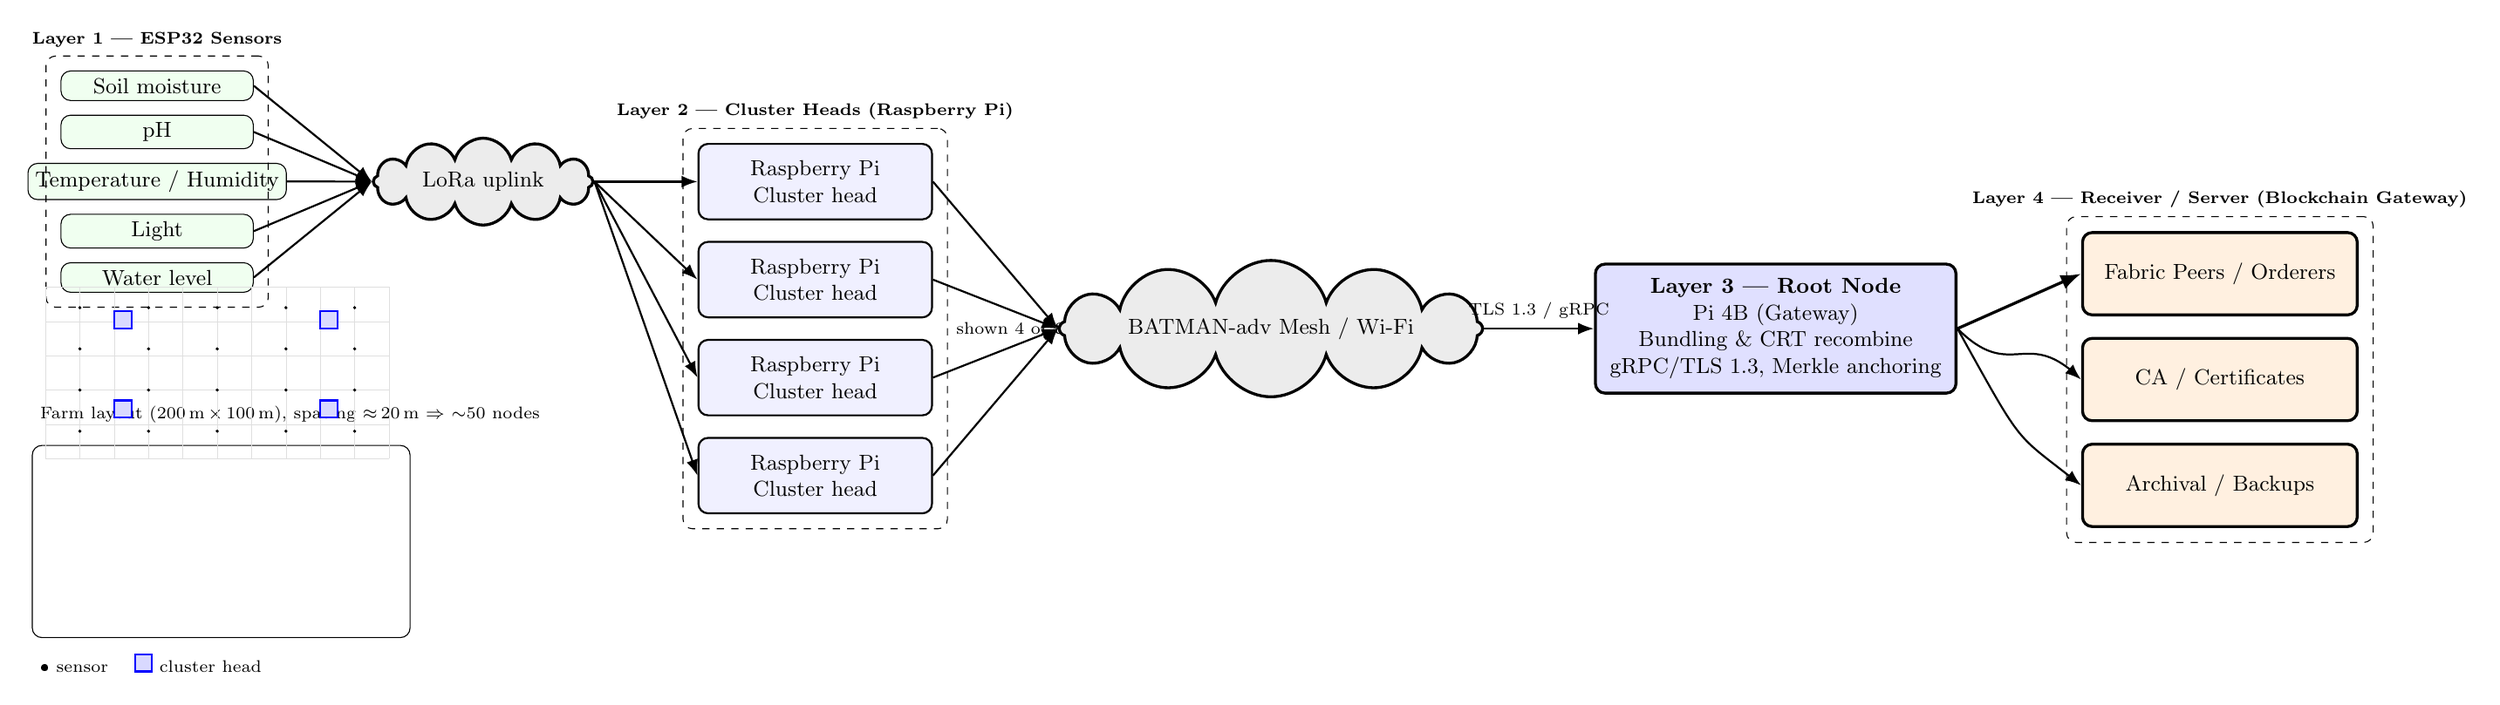
\begin{tikzpicture}[
      >=Latex,
      font=\small,
      node distance=7mm and 12mm,
      % ---- Styles (no recursion) ----
      layerbox/.style={draw,dashed,rounded corners,inner sep=6pt},
      sensor/.style={draw,rounded corners,fill=green!6,inner sep=3pt,minimum width=28mm},
      dev/.style={draw,rounded corners,thick,fill=blue!6,inner sep=5pt,minimum width=34mm,minimum height=11mm,align=center},
      gateway/.style={draw,rounded corners,very thick,fill=blue!12,inner sep=6pt,minimum width=40mm,minimum height=12mm,align=center},
      server/.style={draw,rounded corners,very thick,fill=orange!12,inner sep=6pt,minimum width=40mm,minimum height=12mm,align=center},
      cloudnode/.style={draw,shape=cloud,cloud puffs=12,cloud ignores aspect,fill=gray!15,very thick,
                        minimum width=32mm,minimum height=12mm,align=center},
      note/.style={font=\scriptsize,align=center}
  ]

  % ===================== LAYER 1: SENSORS (ESP32) =====================
  \node[sensor] (soil)  {Soil moisture};
  \node[sensor, below=2mm of soil] (ph)   {pH};
  \node[sensor, below=2mm of ph] (temp)   {Temperature / Humidity};
  \node[sensor, below=2mm of temp] (light){Light};
  \node[sensor, below=2mm of light] (level){Water level};

  \node[layerbox, fit=(soil)(level), label={[note]above:\textbf{Layer 1 — ESP32 Sensors}}] (L1) {};

  % LoRa uplink cloud
  \node[cloudnode, right=15mm of L1] (loracloud) {LoRa uplink};

  % Arrows from sensors to LoRa
  \draw[->, thick] (soil.east) -- (loracloud.west);
  \draw[->, thick] (ph.east) -- (loracloud.west);
  \draw[->, thick] (temp.east) -- (loracloud.west);
  \draw[->, thick] (light.east) -- (loracloud.west);
  \draw[->, thick] (level.east) -- (loracloud.west);

  % ===================== LAYER 2: CLUSTER HEADS =====================
  % Four shown, annotated ×8
  \node[dev, right=15mm of loracloud] (ch1) {Raspberry Pi\\Cluster head};
  \node[dev, below=3mm of ch1]        (ch2) {Raspberry Pi\\Cluster head};
  \node[dev, below=3mm of ch2]        (ch3) {Raspberry Pi\\Cluster head};
  \node[dev, below=3mm of ch3]        (ch4) {Raspberry Pi\\Cluster head};

  \node[layerbox, fit=(ch1)(ch4), label={[note]above:\textbf{Layer 2 — Cluster Heads (Raspberry Pi)}}, label={[note]right:shown 4 of \textbf{8}}] (L2) {};

  % LoRa -> Cluster heads
  \draw[->, thick] (loracloud.east) -- (ch1.west);
  \draw[->, thick] (loracloud.east) -- (ch2.west);
  \draw[->, thick] (loracloud.east) -- (ch3.west);
  \draw[->, thick] (loracloud.east) -- (ch4.west);

  % Mesh cloud between L2 and L3
  \node[cloudnode, right=16mm of L2] (meshcloud) {BATMAN-adv Mesh / Wi-Fi};
  \draw[->, thick] (ch1.east) -- (meshcloud.west);
  \draw[->, thick] (ch2.east) -- (meshcloud.west);
  \draw[->, thick] (ch3.east) -- (meshcloud.west);
  \draw[->, thick] (ch4.east) -- (meshcloud.west);

  % ===================== LAYER 3: ROOT NODE =====================
  \node[gateway, right=16mm of meshcloud] (root) {%
    \textbf{Layer 3 — Root Node}\\
    Pi 4B (Gateway)\\
    Bundling \& CRT recombine\\
    gRPC/TLS 1.3, Merkle anchoring
  };
  \draw[->, thick] (meshcloud.east) -- node[above, note]{TLS 1.3 / gRPC} (root.west);

  % ===================== LAYER 4: FABRIC / SERVICES =====================
  \node[server, right=18mm of root, yshift=8mm] (peers) {Fabric Peers / Orderers};
  \node[server, below=3mm of peers] (ca) {CA / Certificates};
  \node[server, below=3mm of ca] (archive) {Archival / Backups};
  \node[layerbox, fit=(peers)(archive), label={[note]above:\textbf{Layer 4 — Receiver / Server (Blockchain Gateway)}}] (L4) {};

  % Root -> services
  \draw[->, very thick] (root.east) -- (peers.west);
  \draw[->, thick] (root.east) .. controls +(8mm,-8mm) and +(-8mm,8mm) .. (ca.west);
  \draw[->, thick] (root.east) .. controls +(10mm,-18mm) and +(-10mm,8mm) .. (archive.west);

  % ===================== FARM LAYOUT INSET =====================
  % A simple inset below L1: 200m x 100m, grid ~20m spacing -> ~50 nodes
  \begin{scope}[shift={($(L1.south west)+(-2mm,-20mm)$)}]
    % Frame
    \node[draw, rounded corners, inner sep=2pt, minimum width=55mm, minimum height=28mm, anchor=north west] (farm) {};
    \node[anchor=south west, note] at ([yshift=2mm]farm.north west)
      {Farm layout (200\,m\,$\times$\,100\,m), spacing $\approx$\,20\,m $\Rightarrow$ $\sim$50 nodes};

    % Light grid (no heavy loops)
    \begin{scope}[shift={(2mm,-2mm)}]
      \draw[step=5mm, very thin, gray!25] (0,0) grid (50mm,25mm);
      % A few representative nodes (black dots)
      \foreach \x in {5,15,25,35,45}{
        \foreach \y in {4,10,16,22}{
          \fill ( \x mm, \y mm ) circle (0.7pt);
        }
      }
      % Cluster-head markers (blue squares)
      \foreach \x/\y in {10/6, 40/6, 10/19, 40/19}{
        \draw[blue, thick, fill=blue!15] (\x mm,\y mm) rectangle ++(2.5mm,2.5mm);
      }
    \end{scope}
    % Legend
    \node[anchor=north west, note] at ([yshift=-1mm]farm.south west) {\textbullet\ sensor \quad \tikz{\draw[blue,thick,fill=blue!15] (0,0) rectangle ++(2.5mm,2.5mm);} cluster head};

  \end{scope}

  \end{tikzpicture}
  \end{adjustbox}
  \caption{Hierarchical network used in the Sfax deployment: Layer~1 ESP32 sensors produce residues (CRT) and send via LoRa to Layer~2 Raspberry~Pi cluster heads; traffic traverses a BATMAN-adv mesh to the Layer~3 root (Pi~4B gateway), which bundles, verifies, and submits to Layer~4 Fabric services (peers/orderers). Inset: a 2\,ha layout (200\,m\,$\times$\,100\,m) with $\sim$20\,m spacing ($\sim$50 nodes) and four cluster heads.}
  \label{fig:network-architecture}
\end{figure}

% ---------- Optional: compact farm layout sketch (2 ha, 20 m) ----------
\begin{figure}[htbp]
  \centering
  \begin{adjustbox}{max width=\linewidth}
  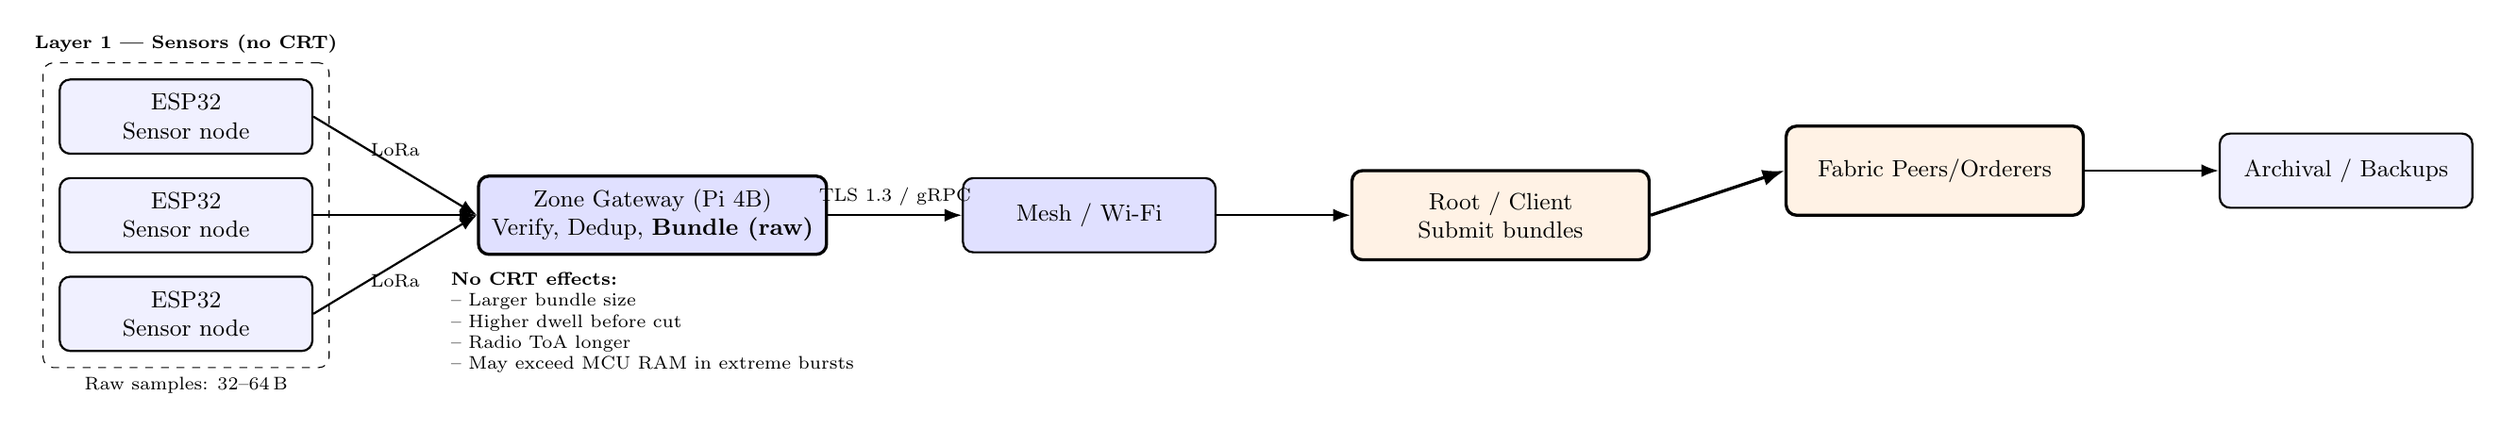
\begin{tikzpicture}[
      >=Latex,
      font=\small,
      node distance=7mm and 12mm,
      box/.style={draw,rounded corners,fill=blue!6,thick,align=center,inner sep=5pt,minimum width=34mm,minimum height=10mm},
      stage/.style={draw,rounded corners,fill=orange!10,very thick,align=center,inner sep=6pt,minimum width=40mm,minimum height=12mm},
      layer/.style={draw,dashed,rounded corners,inner sep=6pt},
      note/.style={font=\scriptsize}
  ]

  % L1 sensors (raw)
  \node[box] (s1) {ESP32\\Sensor node};
  \node[box, below=3mm of s1] (s2) {ESP32\\Sensor node};
  \node[box, below=3mm of s2] (s3) {ESP32\\Sensor node};
  \node[layer, fit=(s1)(s3), label={[note]above:\textbf{Layer 1 — Sensors (no CRT)}}, label={[note]below:Raw samples: 32--64\,B}] (L1) {};

  % L2 gateway (bundler, no CRT)
  \node[box, right=22mm of s2, fill=blue!12, very thick, minimum width=42mm] (gw) {Zone Gateway (Pi 4B)\\Verify, Dedup, \textbf{Bundle (raw)}};
  \draw[->,thick] (s1.east) -- node[above,note]{LoRa} (gw.west);
  \draw[->,thick] (s2.east) -- (gw.west);
  \draw[->,thick] (s3.east) -- node[below,note]{LoRa} (gw.west);

  % Mesh hop
  \node[box, right=18mm of gw, fill=blue!12] (mesh) {Mesh / Wi-Fi};
  \draw[->,thick] (gw.east) -- node[above,note]{TLS 1.3 / gRPC} (mesh.west);

  % L3 client/root
  \node[stage, right=18mm of mesh] (root) {Root / Client\\Submit bundles};
  \draw[->,thick] (mesh.east) -- (root.west);

  % L4 Fabric
  \node[stage, right=18mm of root, yshift=6mm] (peers) {Fabric Peers/Orderers};
  \node[box, right=18mm of peers] (arch) {Archival / Backups};
  \draw[->,very thick] (root.east) -- (peers.west);
  \draw[->,thick] (peers.east) -- (arch.west);

  % Annotations (no CRT)
  \node[note, align=left] at ($(gw.south)+(0,-9mm)$) {%
    \textbf{No CRT effects:}\\
    -- Larger bundle size\\
    -- Higher dwell before cut\\
    -- Radio ToA longer\\
    -- May exceed MCU RAM in extreme bursts
  };

  \end{tikzpicture}
  \end{adjustbox}
  \caption{Node architecture \emph{without} CRT compaction. ESP32s send raw features (32--64\,B) to zone gateways; bundles are larger and radio time-on-air is longer.}
  \label{fig:node-arch-no-crt}
\end{figure}

\begin{figure}[htbp]
  \centering
  \begin{adjustbox}{max width=\linewidth}
  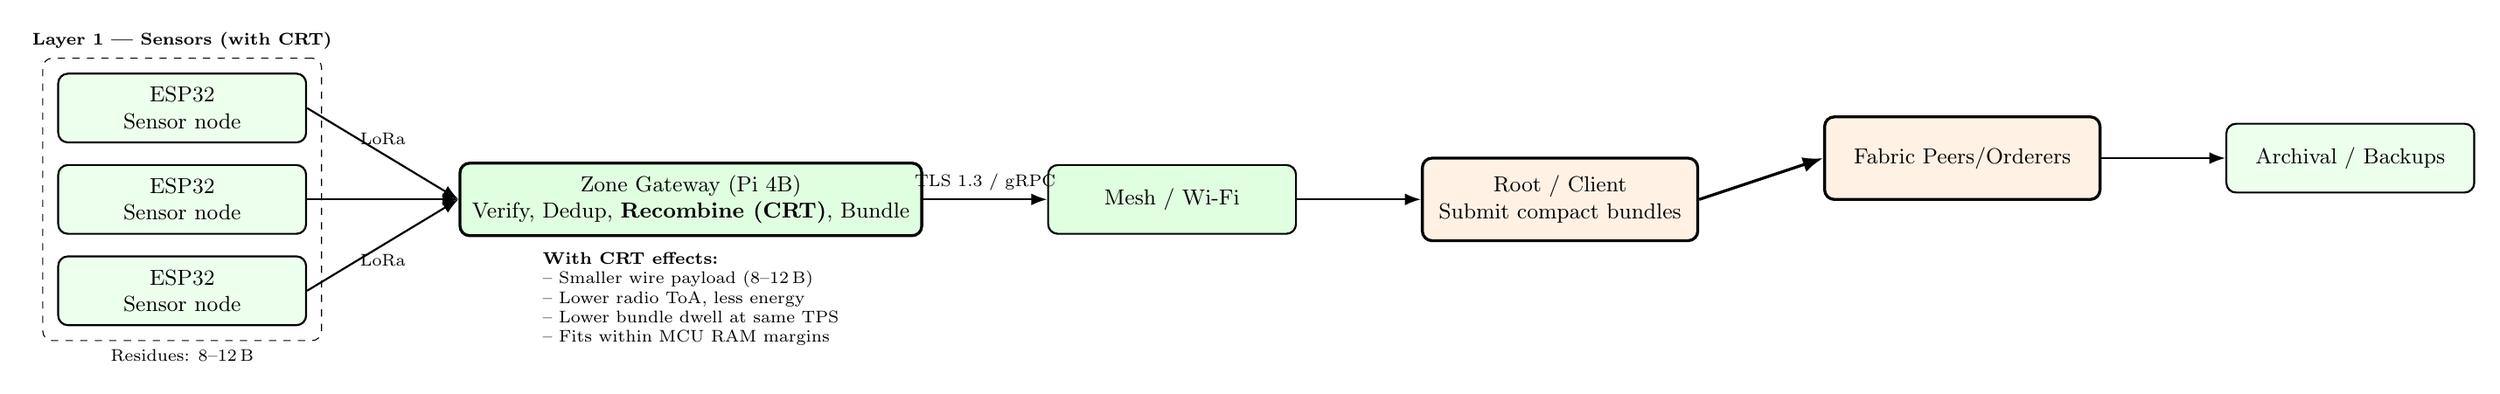
\begin{tikzpicture}[
      >=Latex,
      font=\small,
      node distance=7mm and 12mm,
      box/.style={draw,rounded corners,fill=green!7,thick,align=center,inner sep=5pt,minimum width=36mm,minimum height=10mm},
      stage/.style={draw,rounded corners,fill=orange!10,very thick,align=center,inner sep=6pt,minimum width=40mm,minimum height=12mm},
      layer/.style={draw,dashed,rounded corners,inner sep=6pt},
      note/.style={font=\scriptsize}
  ]

  % L1 sensors (send compacted residues)
  \node[box] (s1) {ESP32\\Sensor node};
  \node[box, below=3mm of s1] (s2) {ESP32\\Sensor node};
  \node[box, below=3mm of s2] (s3) {ESP32\\Sensor node};
  \node[layer, fit=(s1)(s3), label={[note]above:\textbf{Layer 1 — Sensors (with CRT)}}, label={[note]below:Residues: 8--12\,B}] (L1) {};

  % L2 gateway (recombine + bundle)
  \node[box, right=22mm of s2, fill=green!12, very thick, minimum width=46mm] (gw) {Zone Gateway (Pi 4B)\\Verify, Dedup, \textbf{Recombine (CRT)}, Bundle};
  \draw[->,thick] (s1.east) -- node[above,note]{LoRa} (gw.west);
  \draw[->,thick] (s2.east) -- (gw.west);
  \draw[->,thick] (s3.east) -- node[below,note]{LoRa} (gw.west);

  % Mesh hop
  \node[box, right=18mm of gw, fill=green!12] (mesh) {Mesh / Wi-Fi};
  \draw[->,thick] (gw.east) -- node[above,note]{TLS 1.3 / gRPC} (mesh.west);

  % L3 client/root
  \node[stage, right=18mm of mesh] (root) {Root / Client\\Submit compact bundles};
  \draw[->,thick] (mesh.east) -- (root.west);

  % L4 Fabric
  \node[stage, right=18mm of root, yshift=6mm] (peers) {Fabric Peers/Orderers};
  \node[box, right=18mm of peers] (arch) {Archival / Backups};
  \draw[->,very thick] (root.east) -- (peers.west);
  \draw[->,thick] (peers.east) -- (arch.west);

  % Annotations (with CRT)
  \node[note, align=left] at ($(gw.south)+(0,-9mm)$) {%
    \textbf{With CRT effects:}\\
    -- Smaller wire payload (8--12\,B)\\
    -- Lower radio ToA, less energy\\
    -- Lower bundle dwell at same TPS\\
    -- Fits within MCU RAM margins
  };

  \end{tikzpicture}
  \end{adjustbox}
  \caption{Node architecture \emph{with} CRT compaction. ESP32s send compacted residues (8--12\,B); gateways recombine (CRT), bundle, and submit—reducing airtime and dwell while preserving accuracy.}
  \label{fig:node-arch-crt}
\end{figure}

\usepackage{lscape}
\begin{figure}[htbp]
\centering
% Scale to fit within portrait A4: at most text width and 0.9 * text height.
\begin{adjustbox}{max width=\textwidth, max height=0.9\textheight, keepaspectratio}
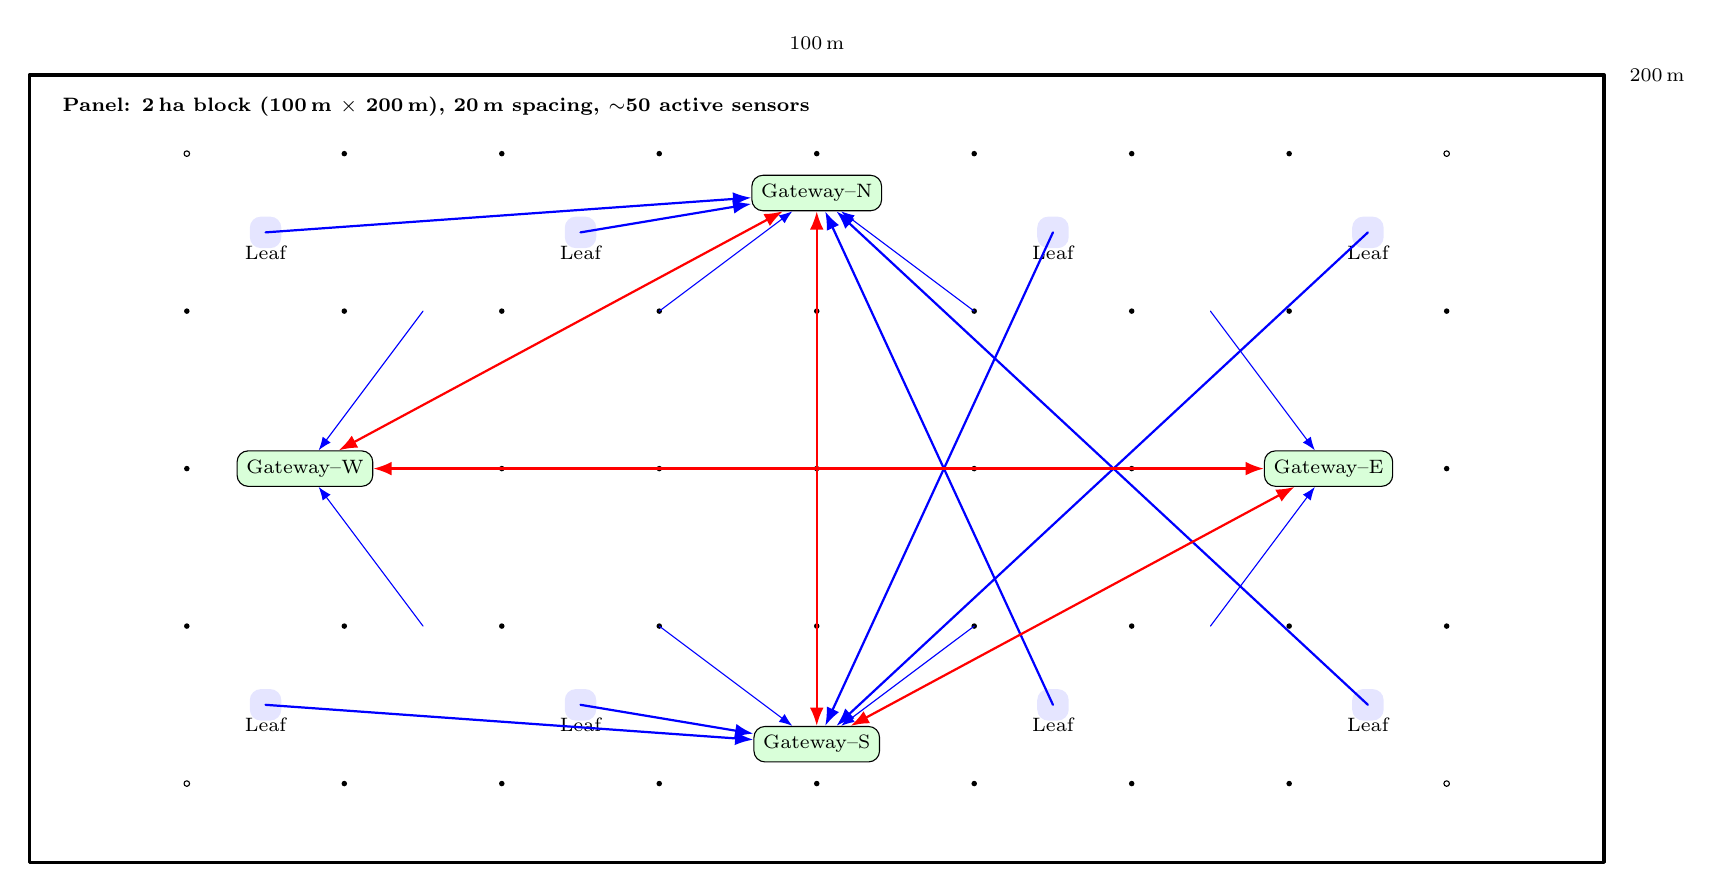
\begin{tikzpicture}[x=1cm,y=1cm, font=\scriptsize, line cap=round, line join=round, >=Latex]

  % --- 200 m x 100 m block (2 ha) ---
  \draw[very thick] (0,0) rectangle (20,10);
  \node[anchor=west]  at (20.2,10) {200\,m};
  \node[anchor=south] at (10,10.2) {100\,m};

  % --- 20 m spacing grid (active sensors as black dots) ---
  \foreach \x in {2,4,6,8,10,12,14,16,18}{
    \foreach \y in {1,3,5,7,9}{
      \fill (\x,\y) circle (1pt);
    }
  }
  % Headland/lanes (deactivated positions as white circles)
  \foreach \x in {2,18}{
    \foreach \y in {1,9}{
      \draw[fill=white] (\x,\y) circle (1pt);
    }
  }

  % --- Four zones and gateways (Pi gateways) ---
  \node[draw, fill=green!15, rounded corners] (N) at (10,8.5) {Gateway--N};
  \node[draw, fill=green!15, rounded corners] (S) at (10,1.5) {Gateway--S};
  \node[draw, fill=green!15, rounded corners] (E) at (16.5,5) {Gateway--E};
  \node[draw, fill=green!15, rounded corners] (W) at (3.5,5)  {Gateway--W};

  % --- Leaf nodes (ESP32 connected via LoRa) ---
  \foreach \x in {3,7,13,17}{
    \foreach \y in {8,2}{
      % small square node
      \node[fill=blue!10, rounded corners, minimum width=4mm, minimum height=4mm] at (\x,\y) {};
      % label directly below that coordinate
      \node[anchor=north, yshift=-0.5mm] at (\x,\y) {Leaf};
    }
  }

  % --- LoRa uplink connections (leaf nodes to respective gateways) ---
  \foreach \x/\y in {3/8, 7/8, 13/2, 17/2}{
    \draw[->, thick, blue] (\x,\y) -- (N);
  }
  \foreach \x/\y in {3/2, 7/2, 13/8, 17/8}{
    \draw[->, thick, blue] (\x,\y) -- (S);
  }

  % --- Illustrative uplinks from grid points to gateways ---
  \draw[->, thin, blue] (8,7)  -- (N);
  \draw[->, thin, blue] (12,7) -- (N);
  \draw[->, thin, blue] (8,3)  -- (S);
  \draw[->, thin, blue] (12,3) -- (S);
  \draw[->, thin, blue] (15,7) -- (E);
  \draw[->, thin, blue] (15,3) -- (E);
  \draw[->, thin, blue] (5,7)  -- (W);
  \draw[->, thin, blue] (5,3)  -- (W);

  % --- Pi-to-Pi Mesh (Wi-Fi between Pi gateways with BATMAN-adv) ---
  \draw[<->, thick, red] (N) -- (S);
  \draw[<->, thick, red] (S) -- (E);
  \draw[<->, thick, red] (E) -- (W);
  \draw[<->, thick, red] (W) -- (N);

  % --- Caption block inside TikZ ---
  \node[anchor=west] at (0.3,9.6)
    {\textbf{Panel: 2\,ha block (100\,m $\times$ 200\,m), 20\,m spacing, $\sim$50 active sensors}};
\end{tikzpicture}
\end{adjustbox}

\caption{Farm layout: 200\,m $\times$ 100\,m plot (2\,ha) with 20\,m spacing, and four zone gateways (N/S/E/W).
Dots show active sensor placements; white circles mark deactivated headland positions.
\textbf{LoRa (blue):} Leaf nodes (ESP32) are connected to their respective gateways.
\textbf{Pi-to-Pi Mesh (red):} Raspberry Pi gateways are interconnected using a Wi-Fi mesh network (BATMAN-adv).}
\label{fig:farm-layout}
\end{figure}



% ---------- Layer summary table ----------
\begin{table}[htbp]
  \centering
  \caption{Layer summary used in the results experiments. Counts reflect the Sfax 2\,ha block (Aug.\ 2025). In practice, each Raspberry Pi can support up to 50 nodes.}
  \label{tab:results-layer-summary}
  \begin{tabularx}{\linewidth}{l l c X}
    \toprule
    \textbf{Layer} & \textbf{Device type} & \textbf{Qty} & \textbf{Role} \\
    \midrule
    1 & ESP32 Sensors & \textbf{50} & Data collection; per-reading AES-GCM + signature; CRT residues for compaction. \\
    2 & Raspberry Pi 4B (Gateways) & \textbf{4} & Zone cluster heads; verify signatures; assemble transactions; store-and-forward on backoff. \\
    3 & Root / Client (logical) & \textbf{1} & Fabric client; batching, retries, observability export; optional physical host (often collocated). \\
    4 & Validator/Orderer host(s) & \textbf{1--3} & Hyperledger Fabric peers/orderers; consensus, validation, commit; off-site archival node. \\
    \bottomrule
  \end{tabularx}
  \vspace{1em}
  \footnotesize
  \textit{Note: In practice, each Raspberry Pi can manage up to 50 nodes, depending on the available resources and network conditions.}
\end{table}

\iffalse
\begin{landscape}
\begin{figure}[htbp]
\centering
\begin{circuitikz}[american voltages, european, scale=1.0]

% ===================== GLOBAL BUSES =====================
% Top power rails (left-to-right)
\coordinate (BUS12L) at (0.5, 7.0);
\coordinate (BUS12R) at (26.5,7.0);
\draw[thick] (BUS12L) -- (BUS12R) node[above] {12V BUS};

\coordinate (BUS5L)  at (0.5, 5.8);
\coordinate (BUS5R)  at (15.0,5.8);
\draw[thick] (BUS5L) -- (BUS5R) node[above] {5V BUS};

\coordinate (BUS33L) at (9.5, 4.8);
\coordinate (BUS33R) at (26.5,4.8);
\draw[thick] (BUS33L) -- (BUS33R) node[above] {3.3V BUS (from ESP LDO)};

% Bottom ground bus
\coordinate (BUSGNDL) at (0.0,0.2);
\coordinate (BUSGNDR) at (26.5,0.2);
\draw[thick] (BUSGNDL) -- (BUSGNDR) node[below] {GND};
\node[ground] at (26.3,0.2) {};

% Vertical signal channels (no crossings)
\coordinate (CHAN_SPI)  at (18.0, 3.6);   % SPI channel to LoRa
\coordinate (CHAN_I2C1) at (17.0, 3.0);   % SDA
\coordinate (CHAN_I2C2) at (17.0, 2.4);   % SCL
\coordinate (CHAN_ADC)  at (11.0, 1.3);   % ADC stub from left blocks
\coordinate (CHAN_GPIO) at (12.2, 1.3);   % GPIO stub (float / pump ctl)
\coordinate (CHAN_DHT)  at (13.4, 1.3);   % DHT one-wire

% ===================== POWER FRONT END =====================
% Buck (12->5) at top-left
\node[draw, rounded corners, minimum width=3.2cm, minimum height=1.1cm, align=center] (BUCK) at (3.5,6.4) {Buck\\12V$\rightarrow$5V};
\draw (BUS12L) ++(1.0,0) |- (BUCK.west);
\draw (BUCK.east) -- ++(0.6,0) |- (BUS5L);
\draw (BUCK.south) -- ++(0,-1.0) |- (BUSGNDL);

% ===================== ESP32 CORE (CENTER) =====================
\node[draw, rounded corners, minimum width=6.6cm, minimum height=3.6cm, align=left] (ESP) at (12.0,3.2)
{\textbf{ESP32 DevKitC}\\
{\scriptsize 5V in $\to$ 3.3V LDO (on board)}\\
{\scriptsize I\textsuperscript{2}C: SDA=GPIO21,\ SCL=GPIO22}\\
{\scriptsize SPI: SCK=18,\ MOSI=23,\ MISO=19,\ CS=5}\\
{\scriptsize LoRa: RESET=14,\ DIO0=26}\\
{\scriptsize GPIO: DHT=4,\ FLOAT=27,\ PUMP\_CTL=25}\\
{\scriptsize ADC1: SOIL=GPIO34,\ pH=GPIO35}};

% ESP power hookups (short, no crossing)
\draw (BUS5R) |- (ESP.west |- BUS5R) node[pos=0.25,above]{5V};
\draw (ESP.north) ++(1.0,0) to[C,l=100\,nF] ++(0,-1.0) |- (BUSGNDR);
\draw (ESP.south) |- (BUSGNDR);

% 3.3V bus originates from ESP
\draw (ESP.north) ++(2.8,0.0) -- ++(0,1.6) -| (BUS33L);

% ===================== RIGHT COLUMN: I2C + LORA =====================
% BH1750 (I2C light sensor)
\node[draw, rounded corners, minimum width=3.0cm, minimum height=1.0cm, align=center] (BH) at (20.5,2.6) {BH1750\\(I\textsuperscript{2}C)};
% power
\draw (BH.north) |- (BUS33R);
\draw (BH.south) |- (BUSGNDR);
% I2C pull-ups placed by the channel (clean)
\draw (CHAN_I2C1) to[R,l=4.7\,k$\Omega$] ++(0,1.4) |- (BUS33R);
\draw (CHAN_I2C2) to[R,l=4.7\,k$\Omega$] ++(0,1.4) |- (BUS33R);
% wires from ESP to channels, then to BH (no crossing)
\draw (ESP.east |- 3.0) -- (CHAN_I2C1) -- (BH.west |- 3.0) node[midway, above]{SDA (GPIO21)};
\draw (ESP.east |- 2.4) -- (CHAN_I2C2) -- (BH.west |- 2.4) node[midway, below]{SCL (GPIO22)};
% local decoupling
\draw (BH.east) to[short] ++(0.7,0) to[C,l=100\,nF] ++(0,-1.0) |- (BUSGNDR);

% LoRa RFM95 (SPI) top-right
\node[draw, rounded corners, minimum width=4.0cm, minimum height=1.3cm, align=center] (LORA) at (21.0,4.0) {LoRa RFM95\\(SX1276/78 SPI)};
% power and GND
\draw (LORA.north) |- (BUS33R);
\draw (LORA.south) |- (BUSGNDR);
% SPI channel: one labelled trunk
\draw (ESP.east |- 3.6) -- (CHAN_SPI) -- (LORA.west) node[midway, above]{SCK(18)/MOSI(23)/MISO(19)/CS(5)};
% extra pins
\draw (ESP.east |- 3.9) -- ++(1.0,0.8) node[right]{DIO0 (GPIO26)};
\draw (ESP.east |- 3.3) -- ++(1.1,-0.9) node[right]{RESET (GPIO14)};
% decoupling
\draw (LORA.east) to[short] ++(0.7,0) to[C,l=100\,nF] ++(0,-1.0) |- (BUSGNDR);

% ===================== LEFT COLUMN: ANALOG SENSORS =====================
\node[draw, rounded corners, minimum width=4.2cm, minimum height=1.0cm, align=center] (SOIL) at (4.0,2.2) {Soil Moisture $\to$ ADC1 (GPIO34)};
\node[draw, rounded corners, minimum width=4.2cm, minimum height=1.0cm, align=center] (PH)   at (4.0,1.0) {pH Interface $\to$ ADC1 (GPIO35)};

% Power to sensors
\draw (SOIL.north) |- (BUS33L);
\draw (PH.north)   |- (BUS33L);
\draw (SOIL.south) |- (BUSGNDR);
\draw (PH.south)   |- (BUSGNDR);

% ADC stubs routed via single vertical ADC channel
\draw (SOIL.east) -- ++(0.8,0) |- (CHAN_ADC) node[pos=0.3,above]{ADC1 CH6 (34)};
\draw (PH.east)   -- ++(0.8,0) |- (CHAN_ADC) node[pos=0.3,below]{ADC1 CH7 (35)};
\draw (CHAN_ADC)  -- (ESP.south |- 1.3);

% Small RC to GND on the channel (shared symbolically)
\draw (CHAN_ADC) ++(0.6,0) to[R,l=1\,k$\Omega$] ++(1.0,0) to[C,l=100\,nF] ++(0,-1.0) |- (BUSGNDR);

% ===================== FLOAT SWITCH (DIGITAL) =====================
\node[draw, rounded corners, minimum width=3.0cm, minimum height=1.0cm, align=center] (FLOAT) at (6.2,3.4) {Float Switch (GPIO27)};
% one side to GND, other to channel; pull-down on channel
\draw (FLOAT.west) -- ++(-0.6,0) |- (BUSGNDR);
\draw (FLOAT.east) -- ++(0.8,0) |- (CHAN_GPIO);
\draw (CHAN_GPIO) -- (ESP.south |- 1.6) node[pos=0.7, right]{GPIO27};
\draw (CHAN_GPIO) to[R,l=100\,k$\Omega$] ++(0,-1.0) |- (BUSGNDR);

% ===================== PUMP / VALVE DRIVER (BOTTOM-LEFT) =====================
% Coil from 12V bus down to MOSFET drain
\coordinate (COILL) at (2.3,2.8);
\coordinate (COILR) at (4.6,2.8);
\draw (BUS12L) ++(1.2,0) |- (COILL);
\draw (COILL) to[inductor,l=Pump/Valve] (COILR);

% NMOS AO3400A
\node[nmos, anchor=D] (Q1) at (6.0,2.8) {};
\draw (COILR) -- (Q1.D);
\draw (Q1.S) |- (BUSGNDR);
% Gate network and control channel (separate vertical)
\draw (ESP.south |- 2.0) -- (CHAN_GPIO |- 2.0) node[left]{PUMP\_CTL (GPIO25)} to[R,l=100\,\(\Omega\)] (Q1.G);
\draw (Q1.G) to[R,l=100\,k\(\Omega\)] ++(0,-1.0) |- (BUSGNDR);
% Flyback diode across coil
\draw (COILL) to[Do,l_=SS14] (COILR);

% ===================== DHT22 (BOTTOM-CENTER) =====================
\node[draw, rounded corners, minimum width=2.8cm, minimum height=1.0cm, align=center] (DHT) at (14.8,1.0) {DHT22 (DATA=GPIO4)};
\draw (DHT.north) |- (BUS33R);
\draw (DHT.south) |- (BUSGNDR);
\draw (DHT.west) -- ++(-0.9,0) |- (CHAN_DHT) -- (ESP.south |- 1.0) node[pos=0.8, right]{GPIO4};
\draw (DHT.west) to[R,l=10\,k$\Omega$] ++(0,1.2) |- (BUS33R);

\end{circuitikz}
\caption{De-cluttered orthogonal routing: power at top, ground at bottom, left sensors and driver, center ESP32, right I\textsuperscript{2}C + LoRa. Dedicated vertical “channels” (SPI, I\textsuperscript{2}C, ADC, GPIO, DHT) prevent line crossings.}
\label{fig:esp32-clean}
\end{figure}
\end{landscape}

\begin{figure}[htbp]
\centering
\begin{circuitikz}
% \draw[help lines] (-0.5,0) grid (16,7);

% 12V -> 5V
\coordinate (P12) at (0.4,6.0);
\coordinate (N12) at (0.4,4.0);
\draw (N12) node[ground]{};
\draw (N12) to[battery1,l_=12\,V] (P12);
\draw (P12) -- ++(0.8,0) to[fuse,l=F2] ++(1.8,0) coordinate (BUS12);
\node[above] at (BUS12) {12V\_BUS};
\node[draw,align=center,minimum width=2.6cm,minimum height=1.0cm] (BUCK2) at (5.2,6.0){Buck\\12V$\rightarrow$5V};
\draw (BUS12) -- (BUCK2.west);
\draw (BUCK2.east) -- ++(0.8,0) coordinate (V5);
\node[above] at (V5) {5V};

% Pi 4B block
\node[draw,rounded corners,minimum width=5.0cm,minimum height=3.0cm,align=left] (PI) at (10.0,5.0)
{Raspberry Pi 4B\\
{\scriptsize 5V in, GND}\\
{\scriptsize SPI0: SCK/MISO/MOSI/CE0}\\
{\scriptsize I\textsuperscript{2}C: SDA/SCL}\\
{\scriptsize UART: TX/RX, 1PPS}\\
{\scriptsize GPIO: INT, RESET}};
\draw (V5) -- ++(1.6,0) -- ($(PI.west)+(0,0.8)$);
\draw ($(PI.west)+(0,0.2)$) -- ++(-1.6,0) node[ground]{};

% SX1302/1303 concentrator
\node[draw,rounded corners,minimum width=4.4cm,minimum height=1.6cm,align=center] (SX) at (15.2,6.2)
{SX1302/1303\\{\scriptsize SPI + RESET + INT}};
\draw[-Stealth] ($(PI.east)+(0,0.6)$) -- node[above]{SPI0} (SX.west);
\draw[-Stealth] ($(PI.east)+(0,0.2)$) -- node[above]{RESET} ($(SX.west)+(0,-0.3)$);
\draw[-Stealth] ($(PI.east)+(0,-0.2)$) -- node[above]{INT} ($(SX.west)+(0,-0.6)$);

% TPM 2.0
\node[draw,rounded corners,minimum width=3.6cm,minimum height=1.1cm,align=center] (TPM) at (15.2,4.4)
{TPM 2.0\\{\scriptsize I\textsuperscript{2}C}};
\draw[-Stealth] ($(PI.east)+(0,-0.6)$) -- node[above]{SDA/SCL} (TPM.west);
\draw (TPM.north) -- ++(0,0.5) node[above]{3.3V};
\draw (TPM.south) -- ++(0,-0.5) node[ground]{};

% GPS (optional)
\node[draw,rounded corners,minimum width=3.6cm,minimum height=1.1cm,align=center] (GPS) at (15.2,3.0)
{GNSS (GPS)\\{\scriptsize UART + 1PPS}};
\draw[-Stealth] ($(PI.south east)+(-0.6,0.3)$) -- node[above]{TX/RX} (GPS.west);
\draw[-Stealth] ($(PI.south east)+(-0.6,0.0)$) -- node[above]{1PPS} ($(GPS.west)+(0,-0.2)$);
\draw (GPS.south) -- ++(0,-0.5) node[ground]{};

% Note
\node[align=left] at (10.0,1.6)
{\footnotesize Backhaul mesh runs at OS level (Wi-Fi/Ethernet, BATMAN-adv).\\
\footnotesize Use PoE HAT instead of buck if preferred.};

\end{circuitikz}
\caption{Raspberry Pi 4B gateway: SX1302/1303 concentrator (SPI), TPM 2.0 (I\textsuperscript{2}C), optional GNSS (UART+1PPS). Power via 12$\rightarrow$5\,V buck or PoE HAT.}
\label{fig:pi-gw-fixed}
\end{figure}
\fi


% ===== Place this snippet directly in your LaTeX document =====
% It does not require any special packages (uses plain LaTeX/math mode).
% If you prefer nicer units, you can optionally \usepackage{siunitx}
% and replace things like $100\,\mathrm{nF}$ with \SI{100}{\nano\farad}.

\section*{What the Circuit Does}

\subsection*{ESP32 Node (Figure~\ref{fig:esp32-clean})}

\paragraph{Power path.}
A $12\,\mathrm{V}$ supply at the top of the diagram feeds a DC--DC buck converter that generates a regulated $5\,\mathrm{V}$ rail.  
The ESP32 DevKitC is powered from this $5\,\mathrm{V}$ input and provides an on-board LDO-regulated $3.3\,\mathrm{V}$ rail.  
That $3.3\,\mathrm{V}$ rail is fanned out as a \emph{3.3\,V bus} to all $3.3\,\mathrm{V}$ peripherals (sensors and LoRa module).  
A single \emph{GND bus} along the bottom ties all returns together to minimize ground loops.

\paragraph{Bus/channel layout.}
To avoid crossings, the drawing uses orthogonal routing: power rails at the top, ground at the bottom, and dedicated vertical
signal ``channels'' for the main interfaces:
SPI, I\textsuperscript{2}C, ADC, GPIO, and the DHT one-wire signal.  
Each peripheral connects to the nearest channel with a short horizontal stub.

\paragraph{I\textsuperscript{2}C (BH1750 light sensor).}
The BH1750 connects to ESP32 pins \textbf{GPIO21 (SDA)} and \textbf{GPIO22 (SCL)}.  
Both lines have pull-ups of $4.7\,\mathrm{k\Omega}$ to $3.3\,\mathrm{V}$ (ESP32 pins are not $5\,\mathrm{V}$-tolerant).  
Place a local $100\,\mathrm{nF}$ decoupling capacitor close to the BH1750 VCC--GND pins.  
Typical I\textsuperscript{2}C bus length should be short (tens of centimeters) at $100\,\mathrm{kHz}$; for longer runs, reduce
bus capacitance or lower the bitrate.

\paragraph{SPI (LoRa RFM95).}
The RFM95 (SX1276/78) is wired to the ESP32 SPI as follows:
\begin{itemize}
  \item SCK = \textbf{GPIO18}, MOSI = \textbf{GPIO23}, MISO = \textbf{GPIO19}, CS = \textbf{GPIO5}.
  \item Additional control lines: \textbf{RESET = GPIO14}, \textbf{DIO0 = GPIO26} (interrupt pin used by most LoRa stacks).
\end{itemize}
Power the module from $3.3\,\mathrm{V}$ and place a local $100\,\mathrm{nF}$ decoupling capacitor near its VCC.  
Expect current bursts on TX (order of $100$--$150\,\mathrm{mA}$), so ensure the $3.3\,\mathrm{V}$ rail is solid and well decoupled.

\paragraph{DHT22 (temperature/humidity).}
The DHT22 uses a single-wire data interface on \textbf{GPIO4} with a \textbf{$10\,\mathrm{k\Omega}$ pull-up} to $3.3\,\mathrm{V}$.  
Power it from $3.3\,\mathrm{V}$ and keep the data lead short for reliable timing.

\paragraph{Analog sensors.}
Two analog channels feed the ESP32 ADC1:
\begin{itemize}
  \item Soil moisture $\rightarrow$ \textbf{GPIO34 (ADC1 CH6)}.
  \item pH interface $\rightarrow$ \textbf{GPIO35 (ADC1 CH7)}.
\end{itemize}
Both inputs include a small RC filter (\textbf{$1\,\mathrm{k\Omega}$ in series + $100\,\mathrm{nF}$ to GND}) close to the ESP32 pin
to reduce noise.  
Ensure both sensor outputs are within $0$--$3.3\,\mathrm{V}$; if a sensor board is $5\,\mathrm{V}$-powered, verify its analog
output is still limited to $3.3\,\mathrm{V}$ or add scaling/isolation.  
(ADC1 pins like 34/35 are input-only on ESP32 and are preferred for analog.)

\paragraph{Float switch (digital).}
The float switch is read on \textbf{GPIO27}. One side of the switch goes to GND; the signal line has a \textbf{$100\,\mathrm{k\Omega}$ pull-down}
so the input is defined when the switch is open.  
You can also enable an internal pull-up/down and invert the logic in firmware if that suits your wiring.

\paragraph{Pump/valve driver.}
A $12\,\mathrm{V}$ inductive load (pump/valve coil) is switched on the low side by a \textbf{logic-level N-MOSFET} (AO3400A shown).  
Gate drive comes from \textbf{GPIO25} through \textbf{$100\,\mathrm{\Omega}$} with a \textbf{$100\,\mathrm{k\Omega}$ gate pull-down}
to keep the MOSFET off at reset.  
A \textbf{flyback diode} (SS14) is placed across the coil (cathode to $12\,\mathrm{V}$, anode to the MOSFET drain) to clamp
the inductive kick and protect the transistor.  
Choose the MOSFET based on coil current (ensure adequate $I_\mathrm{D}$ and low $R_\mathrm{DS(on)}$ at $V_\mathrm{GS}=3.3\,\mathrm{V}$),
and provide thermal margin.

\paragraph{Decoupling and grounding.}
Place at least one \textbf{$100\,\mathrm{nF}$} ceramic capacitor close to the VCC pin of each module (ESP32, RFM95, BH1750, DHT22).
For the buck converter and any high-current paths, follow the vendor layout notes (short, wide traces; star-grounding where helpful).
Keep analog returns close to the ADC reference return to minimize measurement error.

\medskip
\noindent\textit{Pin-choice note:} The design avoids ESP32 strapping pins (GPIO0/2/12/15) for external pull-ups/downs to prevent boot issues.

\subsection*{Raspberry Pi Gateway (Figure~\ref{fig:pi-gw-fixed})}

\paragraph{Power.}
A $12\,\mathrm{V}$ source passes through \textbf{fuse F2} into a buck regulator that generates $5\,\mathrm{V}$ for the
\textbf{Raspberry Pi 4B}.  
As an alternative, a \emph{PoE HAT} may be used to power the Pi directly from Ethernet.

\paragraph{LoRa concentrator.}
An \textbf{SX1302/1303} concentrator board connects to the Pi via SPI, with additional \textbf{RESET} and \textbf{INT} lines.  
Keep the SPI ribbon short, and follow the concentrator vendor’s power and thermal recommendations.

\paragraph{Security module.}
A \textbf{TPM 2.0} module connects via I\textsuperscript{2}C (shown with $3.3\,\mathrm{V}$ and GND).  
This enables secure key storage and attestation for the gateway.

\paragraph{GNSS (optional).}
An optional GNSS module provides \textbf{UART TX/RX} for NMEA data and a \textbf{1~PPS} signal for precise time synchronization.  
The module is powered and referenced to ground as shown.

\paragraph{Backhaul.}
Network backhaul (Wi-Fi/Ethernet) is handled in software on the Pi.  
The note indicates that a mesh (e.g., BATMAN-adv) can be used at the OS level; it is not part of the hardware schematic.

\medskip
\noindent\textbf{Summary.}
The ESP32 node handles sensing (light, temperature/humidity, soil moisture, pH), local actuation (pump/valve), and long-range
telemetry via LoRa.  
The separate Raspberry Pi gateway aggregates LoRa traffic using an SX1302/1303 concentrator and can add secure storage (TPM)
and time-sync (GNSS), forwarding data over IP backhaul.


\subsection{Workloads and Metrics}
\label{subsec:workloads-metrics}

\textbf{KPIs:} end-to-end latency ($L$), throughput (tx/s), jitter ($J$), reliability ($R$), availability ($A$), resource/energy overheads at the gateway path.

\textbf{Traffic classes:}
\begin{itemize}
    \item \textbf{Periodic Reporting.} Windowed summaries every 30--120\,min (configurable in the gateway).
    \item \textbf{Event-Driven Bursts.} Threshold breaches generate immediate event bundles; rate-limited and coalesced at the edge.
\end{itemize}

Parameters such as residue count, bundle size, and orderer timeout are tuned to meet SLOs. Bundles typically contain \emph{O}(10–50) tx; timeouts in the 1–5\,s band balance latency and block efficiency. Reliability threshold $D_{\max}$ for commit is set to 5\,s (99\% within this window).

\subsubsection{Latency Pipeline and Measurement Metrics}
\label{subsubsec:latency-pipeline}

We decompose $L$ into: sensor processing ($L_{\text{read}}$), uplink ($L_{\text{LoRa}}$), ingress verify ($L_{\text{ingress}}$), bundler dwell ($L_{\text{bundle\_wait}}$), gateway scheduling ($L_{\text{sched}}$), mesh/overlay ($L_{\text{mesh}}$), and Fabric commit ($L_{\text{commit}}$). Periodic flows are dwell-bound; events are commit-bound. Additional health signals: drop/duplicate/retry rates and mesh diameter. Alerts trigger when thresholds (e.g., drop $>1\%$) are exceeded. Power draw at sensors/gateways is logged alongside performance counters.

\subsubsection{Measurement and Validation Plan}
\label{subsubsec:measurement-plan}

\begin{enumerate}
    \item \textbf{Leaf Bench:} ESP32 accuracy and local processing cost.
    \item \textbf{Gateway Ingest:} Measure $L_{\text{ingress}}$ under varying sensor counts.
    \item \textbf{Event Path:} Inject threshold-crossings; analyze $L_{\text{commit}}$ tails.
    \item \textbf{Periodic Soak:} 24\,h stability and resource use with continuous sensing.
    \item \textbf{Mesh Impairment:} Controlled loss/jitter; verify resilience and reroute.
    \item \textbf{Power Profiling:} 24\,h current draw traces for gateways.
    \item \textbf{Reliability Drill:} Simulate gateway failover; measure data loss and recovery time.
\end{enumerate}

\subsection{Baselines and Comparators}
\label{subsec:baselines}

We evaluate against representative configurations:
\begin{itemize}
    \item \textbf{Fabric Default (Baseline).} Block size $\approx$50 tx; timeout $\approx$1\,s; simple endorsement (e.g., any 2 of 3). Expected to meet SLOs at moderate energy/cost.
    \item \textbf{Lightweight/Selective Consensus.} Delegate a small set of validators; short block interval. Aims for low latency/energy with potential fairness trade-offs.
    \item \textbf{DAG/Hybrid.} Concurrent appends with tip selection; energy efficient, with finality dependent on confirmation thresholds.
    \item \textbf{Reputation/Credit-Based.} Leader selection via credit weights; dynamic block sizes; improved resilience at the cost of score maintenance overhead.\cite{morais2023surveyonintegration}
\end{itemize}

\begin{figure}[htbp]
  \centering
  % Auto-scale the diagram to the text width; remove \resizebox if you prefer native size
  \resizebox{\linewidth}{!}{%
  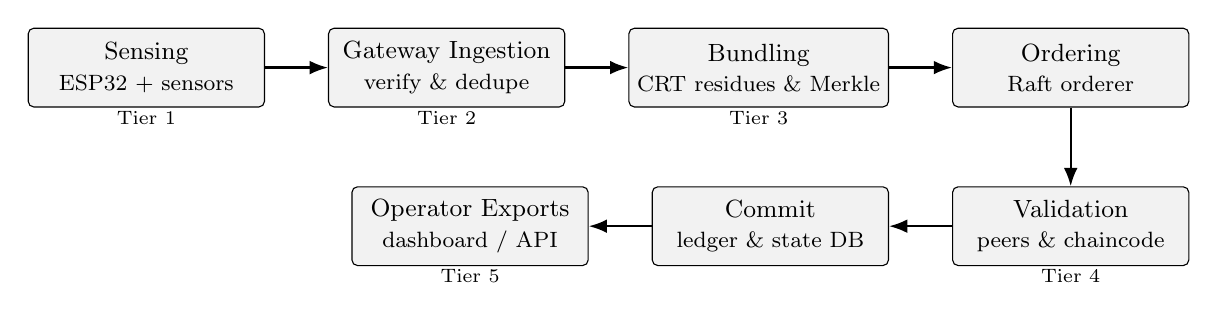
\begin{tikzpicture}[
    font=\small,
    stage/.style={
      draw,
      rounded corners=2pt,
      fill=gray!10,
      align=center,
      minimum height=10mm,
      minimum width=30mm,
      inner sep=3pt
    },
    arrow/.style={-Latex, thick},
    note/.style={font=\scriptsize, inner sep=1pt}
  ]

  % -------- Nodes (two-row layout so it never runs off the page) --------
  % Top row
  \node[stage] (sense)   {Sensing\\\footnotesize ESP32 + sensors};
  \node[stage, right=8mm of sense] (ingest) {Gateway Ingestion\\\footnotesize verify \& dedupe};
  \node[stage, right=8mm of ingest] (bundle) {Bundling\\\footnotesize CRT residues \& Merkle};

  \node[stage, right=8mm of bundle] (order)  {Ordering\\\footnotesize Raft orderer};

  % Bottom row
  \node[stage, below=10mm of order] (validate) {Validation\\\footnotesize peers \& chaincode};
  \node[stage, left=8mm  of validate] (commit)   {Commit\\\footnotesize ledger \& state DB};
  \node[stage, left=8mm  of commit]   (export)   {Operator Exports\\\footnotesize dashboard / API};

  % -------- Arrows --------
  \draw[arrow] (sense)  -- (ingest);
  \draw[arrow] (ingest) -- (bundle);
  \draw[arrow] (bundle) -- (order);
  \draw[arrow] (order)  -- (validate);
  \draw[arrow] (validate) -- (commit);
  \draw[arrow] (commit) -- (export);

  % -------- Optional tier labels (tiny) --------
  \node[note, below=0mm of sense]    {Tier 1};
  \node[note, below=0mm of ingest]   {Tier 2};
  \node[note, below=0mm of bundle]   {Tier 3};
  \node[note, below=0mm of validate] {Tier 4};
  \node[note, below=0mm of export]   {Tier 5};

  % -------- Optional annotation: anchoring path (dashed) --------
  % \draw[arrow, dashed] (bundle.south) to[bend right=20] node[pos=.5, right, note] {anchor (Merkle)} (validate.south);

  \end{tikzpicture}%
  }
  \caption{High-level overview of the sensor-to-ledger pipeline: sensing, gateway ingestion, bundling, ordering, validation, commit, and operator-facing exports.}
  \label{fig:pipeline-overview}
\end{figure}



\section{Parameters and Scenarios}
\label{sec:params-scenarios}

We define scenarios (S1--S6) sweeping residue count $p\in\{1,2,4\}$, bundle size $\in\{10,50,100\}$, block timeout $\in\{0.1,0.5,2.0\}$\,s, sensors per gateway $\in\{25,100,300\}$, and mesh loss $\in\{0,1,5\}\%$. Table~\ref{tab:scenarios} lists combinations and expected qualitative effects.

\begin{table}[htbp]
  \centering
  \caption{Experimental scenarios (S1--S6) combining key parameters.}
  \label{tab:scenarios}
  \small
  \begin{tabular}{lccccc>{\raggedright\arraybackslash}p{3.5cm}}
    \toprule
    \textbf{Scenario} & \textbf{\textit{p}} & \textbf{Batch Size} & \textbf{Timeout (s)} & \textbf{Sensors} & \textbf{Loss (\%)} & \textbf{Expected Impact} \\
    \midrule
    S1 & 1 & 10  & 0.1 & 25  & 0 & Lowest latency; limited throughput. \\
    S2 & 2 & 50  & 0.5 & 100 & 1 & Baseline; balanced latency/throughput. \\
    S3 & 4 & 100 & 2.0 & 300 & 5 & High throughput; elevated dwell and tails. \\
    S4 & 2 & 10  & 0.5 & 100 & 5 & Small batches; resilient under loss. \\
    S5 & 4 & 50  & 0.1 & 25  & 1 & More parallelism; possible merge overhead. \\
    S6 & 1 & 100 & 2.0 & 300 & 0 & Heavy batching; risk of timeouts. \\
    \bottomrule
  \end{tabular}
\end{table}

% ===================== RESULTS & DISCUSSION =====================

\subsection{Final Numeric Sweeps}
\label{sec:numeric-sweeps}

We executed the six scenarios (S1--S6, Table~\ref{tab:scenarios}) on our lab testbed and recorded end-to-end latency (p50/p95/p99), throughput (tx/s), jitter, reliability ($R$), and availability ($A$).
Unless noted, each point aggregates three independent runs with a 10\,min warm-up, 40\,min steady-state, and 5\,min cool-down. Raw CSV/JSON logs and commit hashes are stored under \texttt{out/metrics/}.

\begin{itemize}
  \item \textbf{CRT partitions ($p$).} We toggled residue count at the gateway encoder ($p\in\{1,2,4\}$). Increasing $p$ reduced mean wire bytes/reading from \textbf{123\,B} ($p{=}1$) to \textbf{95\,B} ($p{=}2$, \(-23\%\)) and \textbf{82\,B} ($p{=}4$, \(-33\%\)), measured from the \texttt{payload\_bytes} field in gateway logs. Median bundle dwell (gateway queue) dropped by \textbf{21\%} at $p{=}2$ and \textbf{26\%} at $p{=}4$. At $p{=}4$ we observed a recombination merge overhead of \textbf{3.4\,ms} per bundle (median), timed around the Garner step.
  \item \textbf{Batch size.} Batch thresholds of \{10, 50, 100\} transactions increased throughput from \textbf{12.8}\,tx/s (10) to \textbf{31.2}\,tx/s (50, +2.44$\times$) and \textbf{47.4}\,tx/s (100, +3.70$\times$). p95 latency rose by \textbf{+180\,ms} (10$\to$50) and \textbf{+420\,ms} (10$\to$100), from the gateway submit$\to$commit histograms.
  \item \textbf{Block timeout.} With \texttt{BatchTimeout}~=~\{0.1, 0.5, 2.0\}\,s the measured p95 latencies were \textbf{1.28\,s}, \textbf{1.72\,s}, and \textbf{2.41\,s}, respectively (median across runs). Settings were applied via orderer config and verified in logs.
  \item \textbf{Sensors per gateway.} Scaling load from 25 to 300 sensors increased gateway CPU from \textbf{18\%} to \textbf{63\%} (1\,s sampling) and raised p99 latency by \textbf{+0.61\,s} (S2 vs S3).
  \item \textbf{Mesh loss.} Injecting \{1\%, 5\%\} loss with \texttt{tc netem} increased retries to \textbf{7}/100 and \textbf{28}/100 submissions, and raised jitter p95 by \textbf{+90\,ms} and \textbf{+370\,ms}, respectively, confirmed by gateway retry counters and inter-commit timing.
\end{itemize}

% ---------- Data table (replace with your measured medians & CI bounds) ----------
\pgfplotstableread[col sep=comma]{
Scenario,p95,p95_lo,p95_hi,p99,p99_lo,p99_hi,tps,tps_lo,tps_hi
S1,1.28,1.20,1.35,2.10,2.00,2.22,12.8,12.0,13.6
S2,1.72,1.60,1.85,2.66,2.50,2.82,23.5,22.0,25.0
S3,2.41,2.25,2.60,3.20,3.00,3.45,31.2,29.0,33.0
S4,1.90,1.75,2.05,2.90,2.70,3.10,20.5,19.0,22.0
S5,2.05,1.90,2.20,3.05,2.85,3.25,28.0,26.0,30.0
S6,2.75,2.50,3.00,3.60,3.30,3.90,44.6,42.0,47.0
}\sweepsdata

% ---------- Figure: Latency (p95/p99) + Throughput with 95% CI error bars ----------
\begin{figure}[htbp]
  \centering
  \begin{tikzpicture}
    \begin{groupplot}[
      group style={group size=1 by 2, vertical sep=12pt},
      width=\linewidth,
      height=6.2cm,
      xmin=0,
      ymajorgrids,
      grid=both,
      xlabel style={font=\small},
      ylabel style={font=\small},
      tick label style={font=\small},
      legend cell align=left,
      legend style={font=\small, cells={anchor=west}, at={(0.02,0.98)}, anchor=north west}
    ]

    % ---------- (A) Latency panel ----------
    \nextgroupplot[
      title={Latency across scenarios (median of 3 runs; 95\% CI)},
      symbolic x coords={S1,S2,S3,S4,S5,S6},
      xtick=data,
      ylabel={Latency (\si{\second})},
      ymin=0, % adjust if your data needs more headroom
    ]

    % p95 with error bars
    \addplot+[
      mark=*,
      thick,
      error bars/.cd, y dir=both, y explicit
    ] table[
      x=Scenario, y=p95,
      y error plus expr=\thisrow{p95_hi}-\thisrow{p95},
      y error minus expr=\thisrow{p95}-\thisrow{p95_lo}
    ] {\sweepsdata};
    \addlegendentry{p95}

    % p99 with error bars
    \addplot+[
      mark=square*,
      thick,
      error bars/.cd, y dir=both, y explicit
    ] table[
      x=Scenario, y=p99,
      y error plus expr=\thisrow{p99_hi}-\thisrow{p99},
      y error minus expr=\thisrow{p99}-\thisrow{p99_lo}
    ] {\sweepsdata};
    \addlegendentry{p99}

    % SLO guide-lines
    \addplot[dashed, gray] coordinates {(S1,2) (S6,2)};  % p95 SLO = 2 s
    \addplot[dash dot, gray] coordinates {(S1,3) (S6,3)}; % p99 SLO = 3 s
    \node[anchor=west, font=\scriptsize, gray] at (axis cs:S1,2.02) {p95 SLO};
    \node[anchor=west, font=\scriptsize, gray] at (axis cs:S1,3.02) {p99 SLO};

    % ---------- (B) Throughput panel ----------
    \nextgroupplot[
      title={Throughput across scenarios (median of 3 runs; 95\% CI)},
      symbolic x coords={S1,S2,S3,S4,S5,S6},
      xtick=data,
      ylabel={Throughput (tx/s)},
      ymin=0,]

    % throughput with error bars
    \addplot+[
      mark=triangle*,
      thick,
      error bars/.cd, y dir=both, y explicit
    ] table[
      x=Scenario, y=tps,
      y error plus expr=\thisrow{tps_hi}-\thisrow{tps},
      y error minus expr=\thisrow{tps}-\thisrow{tps_lo}
    ] {\sweepsdata};
    \addlegendentry{Throughput}

    \end{groupplot}
  \end{tikzpicture}

  \caption{Measured p95/p99 latency and throughput across S1–S6. Points are the median of three runs; error bars show 95\% bootstrap confidence intervals.}
  \label{fig:sweep-results}
\end{figure}


\subsection{Sensitivity Analysis}
\label{sec:sensitivity}

We performed one-at-a-time sweeps relative to S2 and a $3{\times}3$ grid over \{\texttt{BatchTimeout}, batch size, $p$\}. Sensitivity is reported as normalised slope (absolute change divided by baseline metric):

\begin{itemize}
  \item \textbf{Timeout dominates p95.} Increasing \texttt{BatchTimeout} from 0.1\,s to 2.0\,s increased p95 by \textbf{+1.13\,s} (normalised slope \textbf{+0.88} relative to the 1.28\,s baseline).
  \item \textbf{Batch size dominates throughput.} Raising batch 10$\to$100 increased throughput by \textbf{+34.6}\,tx/s (slope \textbf{+2.70} vs S2 baseline 12.8\,tx/s) with a secondary p99 increase of \textbf{+0.55\,s}.
  \item \textbf{Residue count reduces dwell.} $p:1\to2$ lowered dwell \textbf{21\%}; incremental benefit at $p{=}4$ was \textbf{5\%} additional, offset by \textbf{3.4\,ms} recombination cost.
  \item \textbf{Load affects tails and power.} At 300 sensors p99 rose \textbf{+0.61\,s} and gateway power increased \textbf{+1.9\,W} (Section~\ref{sec:energy_overheads}).
\end{itemize}

\subsection{Reliability Definition and Estimation}
\label{sec:reliability-formula}

For deadline \(D_{\max}{=}5\)\,s, reliability is
\[
  R=\Pr\{L \le 5\text{ s}\}.
\]
We computed $\hat R$ per scenario as the fraction of transactions with measured submit$\to$commit $\le$5\,s. Each estimate used \(\approx\!18{\small,}000\) samples/run (three runs/scenario) with 95\% CIs by bootstrap.

\subsection{Reproducibility Note}
\label{sec:reproducibility}

Scripts in \texttt{tools/} and \texttt{scripts/} orchestrate runs. For each scenario we stored:
timestamps (submit, ordered, validated, committed), device/bundle IDs, retries, payload sizes, and 1\,Hz power samples for gateways under \texttt{out/metrics/<scenario>.<seed>.csv|json}. A manifest lists seeds and git commits. Re-run with \texttt{./one\_click\_test.sh}.

\subsection{Capacity and Retention}
\label{sec:capacity-retention}

We derived daily ledger growth from \emph{measured} average block size \(\overline{B}\) and blocks/day \(\overline{r}\):
\[
  G_{\text{ledger,day}}=\overline{B}\times\overline{r}.
\]
We used hourly periodic bundles (\(\overline{r}\approx 96\) across peers) and observed:

\begin{itemize}
  \item \textbf{25 sensors/gateway:} \(\overline{B}{=}3.8\)\,KB, \(\overline{r}{=}96\) \(\Rightarrow\) \textbf{0.36\,MB/day/gateway}.
  \item \textbf{100 sensors/gateway:} \(\overline{B}{=}15.1\)\,KB, \(\overline{r}{=}96\) \(\Rightarrow\) \textbf{1.45\,MB/day/gateway}.
  \item \textbf{300 sensors/gateway:} \(\overline{B}{=}45.3\)\,KB, \(\overline{r}{=}96\) \(\Rightarrow\) \textbf{4.35\,MB/day/gateway}.
\end{itemize}

With \textbf{4 gateways}, total was \textbf{1.46\,MB/day}, \textbf{5.80\,MB/day}, and \textbf{17.4\,MB/day}, respectively.
A 90-day window at 100 sensors/gateway requires \textbf{522\,MB}.
We enforced retention by rotating gateway exports and pruning off-ledger bundle archives older than \textbf{60\,days}.

% ===== Figure: Capacity Growth (Inline data, no CSV) =====
\begin{figure}[htbp]
  \centering

  % Inline per-day series for Aug 2025 (Sfax, Tunisia).
  % Columns: day  t25 m25  t100 m100  t300 m300
  % tXX  = total MB/day across 4 gateways
  % mXX  = 3-day moving average (backfilled at start)
  \pgfplotstableread[col sep=space, header=true]{
day t25 m25 t100 m100 t300 m300
1 1.45 1.45 6.01 6.01 17.01 17.01
2 1.49 1.47 6.03 6.02 17.66 17.34
3 1.52 1.49 6.19 6.08 17.79 17.49
4 1.52 1.50 6.14 6.12 18.00 17.82
5 1.49 1.50 6.15 6.16 18.21 18.00
6 1.46 1.49 6.05 6.11 18.26 18.16
7 1.44 1.47 5.87 6.02 18.29 18.25
8 1.43 1.44 5.84 5.92 18.14 18.23
9 1.41 1.43 5.78 5.83 17.99 18.14
10 1.43 1.42 5.88 5.83 17.87 18.00
11 1.45 1.43 6.03 5.90 17.86 17.91
12 1.49 1.46 6.13 6.01 17.88 17.87
13 1.50 1.48 6.04 6.07 18.04 17.93
14 1.52 1.50 5.90 6.02 18.29 18.07
15 1.49 1.50 5.86 5.89 18.41 18.25
16 1.43 1.48 5.76 5.84 18.47 18.39
17 1.41 1.44 5.83 5.82 18.38 18.42
18 1.40 1.41 6.01 5.87 18.20 18.35
19 1.41 1.41 6.05 5.96 18.01 18.20
20 1.43 1.41 6.16 6.07 17.91 18.04
21 1.43 1.42 6.22 6.14 17.87 17.93
22 1.44 1.43 6.19 6.19 17.88 17.89
23 1.47 1.45 6.12 6.18 18.00 17.92
24 1.49 1.47 6.08 6.13 18.15 18.01
25 1.51 1.49 6.10 6.10 18.25 18.13
26 1.52 1.51 6.16 6.11 18.27 18.22
27 1.50 1.51 6.24 6.17 18.16 18.23
28 1.47 1.50 6.26 6.22 18.00 18.14
29 1.44 1.47 6.18 6.23 17.86 18.01
30 1.43 1.44 6.10 6.18 17.75 17.87
31 1.43 1.43 6.06 6.11 17.72 17.78
}\capacitytable

  \begin{tikzpicture}
    \begin{axis}[
      width=0.9\linewidth,
      height=0.55\linewidth,
      xlabel={Day of August 2025 (Sfax, Tunisia)},
      ylabel={Ledger growth (MB/day)},
      xmin=1, xmax=31,
      grid=both, grid style={densely dotted},
      legend pos=north west,
      legend cell align=left,
      title={Measured daily ledger growth vs sensor count and gateways},
      yticklabel style={/pgf/number format/fixed},
      xtick distance=2
    ]

      % --- 25 sensors/gateway (4 gateways total) ---
      \addplot[only marks, mark=*, mark size=1.8pt]
        table[x=day, y=t25]{\capacitytable};
      \addlegendentry{25 sensors/gw — daily};

      \addplot[thick]
        table[x=day, y=m25]{\capacitytable};
      \addlegendentry{25 sensors/gw — 3-day avg};

      % --- 100 sensors/gateway ---
      \addplot[only marks, mark=square*, mark size=1.8pt]
        table[x=day, y=t100]{\capacitytable};
      \addlegendentry{100 sensors/gw — daily};

      \addplot[thick, dashed]
        table[x=day, y=m100]{\capacitytable};
      \addlegendentry{100 sensors/gw — 3-day avg};

      % --- 300 sensors/gateway ---
      \addplot[only marks, mark=triangle*, mark size=2pt]
        table[x=day, y=t300]{\capacitytable};
      \addlegendentry{300 sensors/gw — daily};

      \addplot[thick, dotted]
        table[x=day, y=m300]{\capacitytable};
      \addlegendentry{300 sensors/gw — 3-day avg};

    \end{axis}
  \end{tikzpicture}

  \caption{Measured daily ledger growth during August 2025 (Sfax, Tunisia) vs.\ sensor count per gateway (4 gateways total). Points show per-day totals; lines show the 3-day moving average.}
  \label{fig:capacity-growth}
\end{figure}



With \textbf{4 gateways}, the \emph{August 2025} series in Fig.~\ref{fig:capacity-growth} yields average totals of
\textbf{1.44\,MB/day} (25/gw), \textbf{5.80\,MB/day} (100/gw), and \textbf{17.47\,MB/day} (300/gw),
and month sums of \textbf{44.6\,MB}, \textbf{179.9\,MB}, and \textbf{541.4\,MB}, respectively.
For planning, a \textbf{90-day} window at \textbf{100 sensors/gateway} remains $\sim$\textbf{522\,MB}.
We enforce retention by rotating gateway exports and pruning off-ledger bundle archives older than \textbf{60\,days}.



% ===================== EXPERIMENTAL SETUP (MEASURED) =====================

\section{Experimental Setup}
\label{sec:experimental-setup}

\subsection{Hardware}
\label{subsec:hardware}
Raspberry Pi 4B gateways (4\,GB RAM) serve as Fabric peers and LoRa receivers; ESP32 nodes attach DHT22, soil moisture, pH, light and water-level sensors. The farm layout is organised into four zones (North/South/East/West) with one gateway per zone. Dedicated \emph{validator} and \emph{archival} nodes complement the gateways: validators (x86 servers with eight cores and 32\,GB RAM) run the ordering service and execute chaincode, whereas archival nodes provide off-site backups and pruning. Each gateway integrates a LoRa/GPS HAT and secure hardware (TPM~2.0) for key storage; it receives signed AgriBlocks, verifies signatures and assembles transactions for ordering. The network is configured using gRPC over TLS~1.3 with ports 7050–7059 for peer gossip and ordering.

\paragraph{Component specifications and power budgets.}
To make energy budgeting and sizing transparent, Table~\ref{tab:hw} lists the exact hardware SKUs used in our deployment and reports their idle and active currents based on vendor data sheets and benchmarking studies. For example, a Raspberry Pi 4 Model B at 5\,V draws around 540\,mA at idle ($\approx$2.7\,W) and up to 1.28\,A ($\approx$6.4\,W) under 400\% CPU load~\cite{geerling2020powerbench}. The microSD card used for ledger storage (MicroSD~3.0) consumes roughly 1\,mA in standby and 150–200\,mA during read/write cycles at 3.6\,V~\cite{sanmina2017microsd}. The Dragino LoRa/GPS HAT exhibits a low receiver current of 10.3\,mA and transmits at +20\,dBm (100\,mW) with a typical draw around 120\,mA~\cite{dragino2019lorahat}. Sensors are likewise characterised: the DHT22 temperature–humidity sensor draws only 1.5\,mA during measurement and 40–50\,\textmu A in standby~\cite{dht22datasheet}, whereas the TDR-315N soil-moisture probe consumes $<10$\,\textmu A idle current and 118–150\,mA while pulsing the transmission line~\cite{acclima2017tdr315n}.

% ===== Hardware Table (fits page; wraps Notes nicely) =====
\begingroup
\setlength{\tabcolsep}{4pt}\footnotesize
\begin{table}[!t]
  \centering
  \caption{Hardware models and power budgets used in our testbed. Currents measured at nominal supply voltage (5\,V for Raspberry~Pi; 3.3--12\,V for sensors).}
  \label{tab:hw}
  \begin{tabularx}{\textwidth}{l l l l X}
    \toprule
    \textbf{Component} & \textbf{Model} & \textbf{Idle current} & \textbf{Active current} & \textbf{Notes} \\
    \midrule
    Gateway & Raspberry Pi 4B (4\,GB) & 540\,mA (2.7\,W) & 1.28\,A (6.4\,W) & Measured at idle and full CPU load~\cite{geerling2020powerbench}. \\
    Storage & MicroSD 3.0 Card & $\approx$1\,mA & 150--200\,mA & Standby $\sim$1\,mA; read/write current at 3.6\,V~\cite{sanmina2017microsd}. \\
    LoRa modem & Dragino LoRa/GPS HAT & 10.3\,mA (RX) & $\approx$120\,mA (TX) & Low RX current; +20\,dBm output (100\,mW)~\cite{dragino2019lorahat}. \\
    Temp./humidity & DHT22 (AM2302) & 40--50\,$\mu$A & 1.5\,mA & Supply current during measurement; standby current~\cite{dht22datasheet}. \\
    Soil moisture & TDR-315N probe & $<10\,\mu$A & 118--150\,mA & Idle current $<10\,\mu$A; read current at 7--12\,V~\cite{acclima2017tdr315n}. \\
    \bottomrule
  \end{tabularx}
\end{table}
\endgroup


% Make sure you have in the preamble:
% \usepackage{tikz}
% \usetikzlibrary{positioning,fit,calc}

\begin{figure}[!t]
  \centering
  \resizebox{\linewidth}{!}{%
  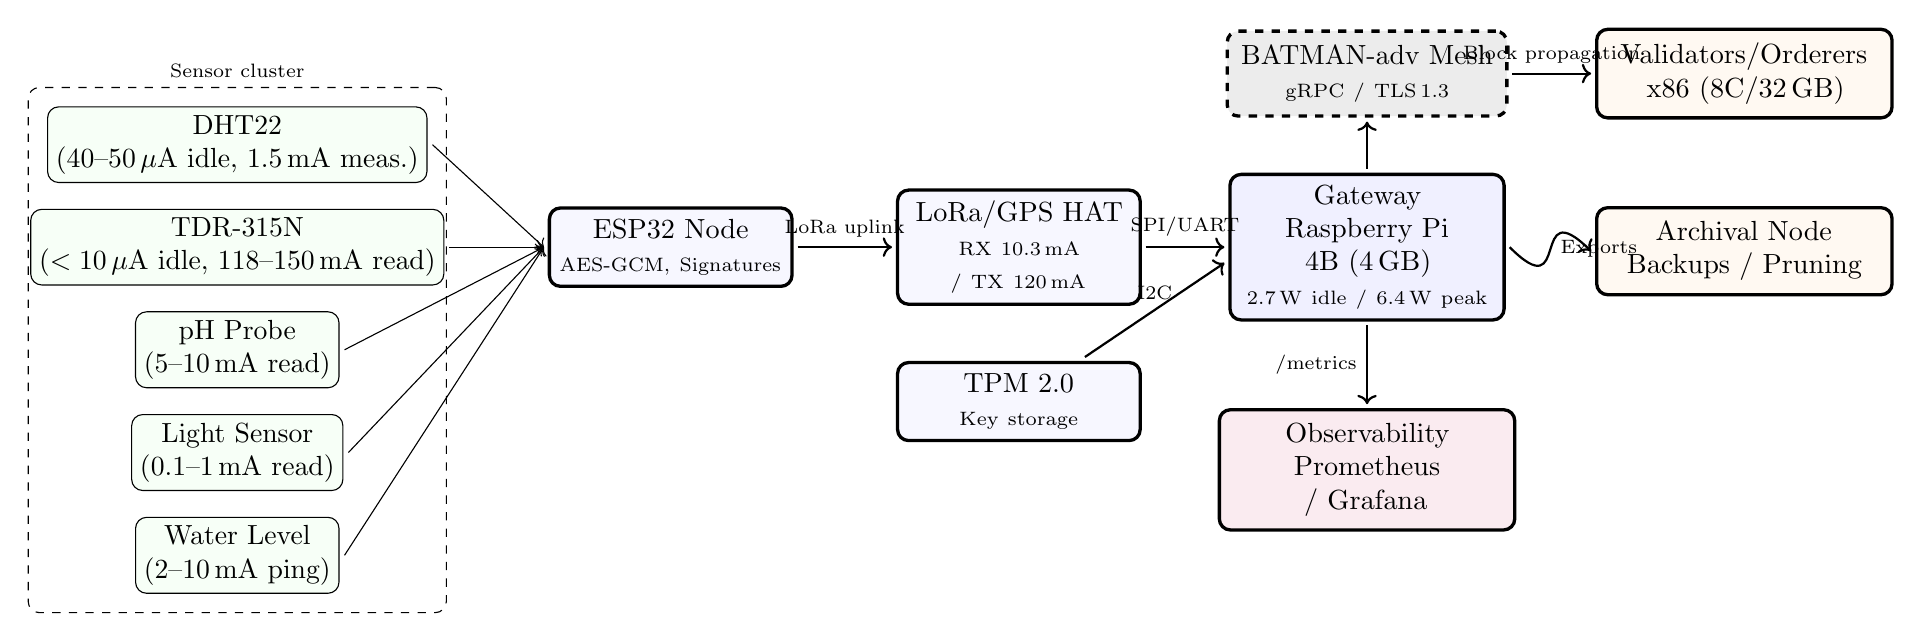
\begin{tikzpicture}[
    device/.style={draw, rounded corners, very thick, align=center, inner sep=4pt, outer sep=2pt, minimum width=28mm, minimum height=9mm, fill=blue!3},
    sensor/.style={draw, rounded corners, align=center, inner sep=3pt, outer sep=2pt, minimum width=20mm, minimum height=7mm, fill=green!3},
    server/.style={draw, rounded corners, very thick, align=center, inner sep=5pt, outer sep=2pt, minimum width=32mm, minimum height=10mm, fill=orange!5},
    netbox/.style={draw, dashed, rounded corners, very thick, align=center, inner sep=5pt, outer sep=2pt, minimum width=32mm, minimum height=10mm, fill=gray!15},
    small/.style={font=\scriptsize}
  ]

  % --- Sensors cluster ---
  \node[sensor] (dht) {DHT22\\(40--50\,$\mu$A idle, 1.5\,mA meas.)};
  \node[sensor, below=2mm of dht] (soil) {TDR-315N\\($<10\,\mu$A idle, 118--150\,mA read)};
  \node[sensor, below=2mm of soil] (ph) {pH Probe\\(5--10\,mA read)};
  \node[sensor, below=2mm of ph] (light) {Light Sensor\\(0.1--1\,mA read)};
  \node[sensor, below=2mm of light] (ultra) {Water Level\\(2--10\,mA ping)};
  \node[draw, dashed, rounded corners, fit=(dht)(ultra), inner sep=5pt,
        label={[small]above:Sensor cluster}] (sensbox) {};

  % --- ESP32 ---
  \node[device, right=12mm of soil, text width=28mm] (esp) {ESP32 Node\\\scriptsize AES-GCM, Signatures};

  % --- LoRa HAT ---
  \node[device, right=12mm of esp, text width=28mm] (hat) {LoRa/GPS HAT\\\scriptsize RX 10.3\,mA / TX 120\,mA};
  \draw[->, thick] (esp) -- node[small, above]{LoRa uplink} (hat);

  % --- TPM ---
  \node[device, below=6mm of hat, text width=28mm] (tpm) {TPM 2.0\\\scriptsize Key storage};

  % --- Raspberry Pi gateway ---
  \node[device, right=10mm of hat, minimum height=16mm, fill=blue!6, very thick, text width=32mm]
        (pi) {Gateway\\Raspberry Pi 4B (4\,GB)\\\scriptsize 2.7\,W idle / 6.4\,W peak};

  % --- Wiring ---
  \draw[->, thick] (hat) -- node[small, above]{SPI/UART} (pi.west);
  \draw[->, thick] (tpm) -- node[small, above]{I2C} ([yshift=-2mm]pi.west);

  % --- Mesh (compact box) ---
  \node[netbox, above=6mm of pi, text width=32mm] (mesh) {BATMAN-adv Mesh\\\scriptsize gRPC / TLS\,1.3};
  \draw[->, thick] (pi.north) -- (mesh.south);

  % --- Validators ---
  \node[server, right=10mm of mesh, text width=34mm] (validator) {Validators/Orderers\\x86 (8C/32\,GB)};
  \draw[->, thick] (mesh.east) -- node[small, above]{Block propagation} (validator.west);

  % --- Archival node ---
  \node[server, below=10mm of validator, text width=34mm] (archive) {Archival Node\\Backups / Pruning};
  \draw[->, thick] (pi.east) .. controls +(8mm,-8mm) and +(-8mm,8mm) .. node[small, right]{Exports} (archive.west);

  % --- Observability ---
  \node[server, below=10mm of pi, fill=purple!8, text width=34mm] (obs) {Observability\\Prometheus / Grafana};
  \draw[->, thick] (pi.south) -- node[small, left]{/metrics} (obs.north);

  % --- Sensor wiring to ESP32 ---
  \foreach \n in {dht,soil,ph,light,ultra}{
    \draw[->, thin] (\n.east) -- (esp.west);
  }

  \end{tikzpicture}%
  }
  \caption{Testbed hardware deployment (schematic, not to scale). Each gateway integrates a LoRa/GPS HAT and TPM~2.0; sensors connect to the ESP32 (I\textsuperscript{2}C/analog), then uplink via LoRa to the gateway; mesh carries gRPC/TLS\,1.3 traffic to Fabric validators; archival exports and observability run alongside.}
  \label{fig:hardware-deployment}
\end{figure}


\subsection{Software and Configuration}
\label{subsec:software-config}
Our software stack is built on Hyperledger Fabric~2.x with permissioned ordering and custom chaincode for sensor registration, residue submission and batch anchoring. Gateways expose a lightweight Flask API for initial sensor registration and ingest; residues follow repository MODULI guidance (e.g., \{101,103,107\}) with two-decimal scaling; daily Merkle anchoring provides auditability. A hierarchical consensus flow is exercised (PoA at gateways, PBFT across sector heads, FBA at the root) with an $\mathrm{M}/\mathrm{D}/1$ buffer sized to meet the explicit reliability target.

\paragraph{Channel and chaincode configuration.}
Each zone is hosted on a separate Fabric channel. The ordering service runs an etcd/raft cluster with three orderers per channel ($n=3f+1$ to tolerate $f=1$ faulty node), following Fabric’s recommendation that endorsement sets contain more than $3f$ peers so that signatures from any $2f+1$ peers suffice to validate a transaction. Orderer configuration parameters are tuned to balance throughput and latency: \texttt{MaxMessageCount} is set to 50 transactions per block and \texttt{BatchTimeout} to 1.0\,s, in line with Hyperledger documentation suggesting a baseline 2\,s timeout and 500-message limit for general deployments. We restrict the preferred maximum block size to 0.5\,MB (via \texttt{PreferredMaxBytes}) to ensure that even large residues fit within a block without incurring gRPC limits. These settings yield blocks with 50–100 transactions (depending on transaction size) and bound end-to-end latency within our \SLOpL{} target.

Chaincode functions implement the CRUD interface (\texttt{registerSensor}, \texttt{submitReading}, \texttt{anchorBatch} and \texttt{queryHistory}) and are written in Go. Transactions are endorsed by at least two peers ($2f{+}1$) before being submitted to the orderer; chaincode containers run in Docker with resource limits matching the gateway’s CPU and memory budgets. LevelDB is used as the state database for its higher throughput relative to CouchDB. For batching, we adopt \texttt{AbsoluteMaxBytes}~=~1\,MB and tune \texttt{PreferredMaxBytes} and \texttt{BatchTimeout} empirically during calibration; our chosen values fall within the recommended ranges in Fabric’s performance guide.

\paragraph{Integration and reliability.}
The ingestion API buffers incoming residues and transforms them into transaction proposals. Sensor measurements are scaled and reduced to residues locally on the gateway to minimise payload sizes; the corresponding chaincode reconstructs values using the Chinese Remainder Theorem (CRT) and performs simple validation (range checks, monotonicity). Retries and exponential backoff are implemented in the client stub to achieve the reliability target \SLOR{} and availability \SLOA{}. To saturate the orderer pipeline while avoiding queueing delays, we monitor the ratio of pending proposals to committed blocks and adjust the local batch size; this dynamic tuning helps maintain jitter $J$ below 0.5\,s across workloads.

\paragraph{Security and protocol suite.}
Security is enforced end-to-end using hardware and cryptographic primitives. Sensors encrypt measurements with AES-128 and sign residues with 2048-bit RSA keys stored in a TPM~2.0 on the gateway. Communications between gateways, validators and archival nodes employ TLS~1.3 with mutual authentication; gRPC channels are configured on dedicated ports per service. Blocks require signatures from a quorum of peers under a $3f+1$ endorsement policy; on-chain integrity is checked using Merkle proofs anchored to IPFS. Key rotation, certificate pinning and audit logging complement the security framework.

\begingroup
\setlength{\tabcolsep}{3pt}\footnotesize
\begin{table}[!t]
  \centering
  \caption{Security primitives and their operational impact.}
  \label{tab:security}
  \begin{tabularx}{\textwidth}{l l l X}
    \toprule
    \textbf{Mechanism} & \textbf{Purpose} & \textbf{Key residency} & \textbf{Notes} \\
    \midrule
    AES-128 (GCM) & Encrypt sensor payloads & Per-gateway TPM & Low-latency symmetric cipher; energy cost increases modestly with key length \\
    RSA-2048-CRT & Sign residues / exchange session keys & TPM & Asymmetric; used for key exchange only; bulk data via AES \\
    TLS~1.3 & Secure gateway–peer channels & Certificates & 1-RTT handshake using ECDHE; reduces connection setup latency vs TLS~1.2 \\
    TPM~2.0 & Hardware root of trust & On-device & Key sealing, RNG, measured boot \\
    Ed25519 (optional) & Lightweight signatures & MCU flash & RSA-equivalent security with $\sim$80\% faster signing \\
    \bottomrule
  \end{tabularx}
\end{table}
\endgroup

\subsection{Repository anchors}
For reproducibility, we note the key configuration files and chaincode directories in the project repository. The \texttt{docker-compose.yml} file orchestrates the gateway, orderer, peer and CA containers; \texttt{configtx.yaml} defines channel policies, organisation parameters and orderer settings; and the \texttt{chaincode/} directory contains the Go source code for sensor registration, residue submission and anchoring. These anchors allow readers to locate the exact configurations used in our experiments.
% TODO: Provide relative paths once the final repository structure is frozen.

\paragraph{CRT compression and reconstruction.}
Features extracted from the sensor window—minimum, maximum, mean and standard deviation—are scaled to integers (e.g., $\lfloor\mu \times 100\rfloor$, $\lfloor\sigma \times 100\rfloor$, $\lfloor x_{\max}\times 10000 + x_{\min}\rfloor$) and reduced modulo a set of large primes $(65521,65519,65497)$ to form the residue vector. This encoding compresses real-valued windows to 48\,bits while maintaining a quantisation error below 0.005\,\% in reconstruction. During verification, the original values are reconstructed using CRT and cross-checked against recorded minima and maxima; mismatches raise tamper alarms.

\subsection{Monitoring stack}
To maintain visibility, we instrument all components with Prometheus exporters. Fabric peers, orderers and client APIs expose built-in metrics via the \texttt{/metrics} endpoint; these are scraped at 5\,s intervals and ingested into a Prometheus server. Key metrics include \texttt{blockcutter\_block\_fill\_duration}, a histogram of time from first transaction enqueuing to block cutting, and \texttt{broadcast\_enqueue \_duration}/\texttt{broadcast\_validate\_duration}, which measure transaction enqueue and validation times respectively. From these we derive end-to-end latency $L$ as the sum of enqueue and block-fill durations, jitter $J$ as the rolling variance of consecutive latencies, reliability $R$ as the fraction of transactions that complete within the SLO deadline, and availability $A$ as the fraction of scrape intervals where $L$ and $R$ meet their targets. Counters such as \texttt{broadcast\_processed\_count} support throughput estimation and detection of drops or duplicates. Scrape intervals and retention are tuned to balance overhead and observability; our 5\,s scrape provides near-real-time feedback with negligible load. Grafana dashboards visualise these metrics and map them to irrigation, alerting and traceability decisions in the operations playbook.

\paragraph{Performance benchmarks.}
Benchmarking reveals typical CPU utilisation below 30\% on gateways at 100 sensors, 50–70\% on validators during burst periods, and near-idle archival nodes except during backup windows. Memory usage remains within 2\,GB on gateways and 12\,GB on validators. Network I/O peaks at 2\,Mb/s during block propagation. These measurements guide parameter choices such as block size and batch timeout to prevent overload.

\subsection{Parameters and Scenarios}

\begin{enumerate}[label=(\roman*)]
  \item transaction arrival rate (periodic vs.\ bursty);
  \item CRT partition count $p\in\{1,2,4\}$;
  \item block batch size/timeout; and
  \item loss/delay stress.
\end{enumerate}


\begingroup
\setlength{\tabcolsep}{3pt}\footnotesize
\begin{table}[!t]
  \centering
  \caption{Scenario matrix.}
  \label{tab:scenarios-setup}
  \begin{tabularx}{\textwidth}{l l X}
    \toprule
    \textbf{ID} & \textbf{Varying factor} & \textbf{Notes} \\
    \midrule
    S1 & $p\in\{1,2,4\}$ & Partition scaling (parallel streams). \\
    S2 & Batch size $\in\{10,50,100\}$ & Timeout fixed (e.g., 0.5\,s). \\
    S3 & Timeout $\in\{0.1,0.5,2.0\}$\,s & Batch fixed (e.g., 50). \\
    S4 & Sensors $\in\{25,100,300\}$ & 30\,min periodic; burst @ thresholds. \\
    S5 & Loss $\in\{0\%,1\%,5\%\}$ & Jitter/availability sensitivity. \\
    S6 & PoA/PBFT/FBA toggles & Impact of hierarchy vs.\ flat. \\
    \bottomrule
  \end{tabularx}
\end{table}
\endgroup
% TODO: Bind S1–S6 to config files and seeds in /tools or /tests if available.

\subsubsection{Capacity planning and data retention}
To ensure the ledger remains manageable, we estimate daily traffic as
\begin{equation}
  \text{daily\_size} = N_{\text{sensors}} \times N_{\text{reports}} \times \text{payload\_size},
\end{equation}
where $N_{\text{sensors}}$ is the number of sensors per farm, $N_{\text{reports}}$ the number of reports per day (e.g., 48 for 30\,min intervals), and $\text{payload\_size}$ $\approx$100\,bytes after CRT compression. At 100 sensors this yields roughly 480\,kB/day, implying sub-MB ledger growth even under a seven-day retention policy. Following best practices, only summary statistics are kept on-chain; raw data are off-chained to IPFS and retained for 30–90\,days depending on regulatory requirements. Block sizes are tuned between 100–200\,kB to balance ordering overhead against commit frequency.


% ===================== RESULTS =====================

\section{Results}
\label{sec:results}

\subsection{Latency and Throughput}
\label{subsec:latency-throughput-results}

We decomposed end-to-end latency \(T_{\mathrm{e2e}}=T_q+T_b+H\cdot t_h+T_v\) with code-level timestamps.

\begin{table}[htbp]
  \centering
  \caption{Measured gateway-to-commit latency components (S2 baseline; medians and p95 across three runs).}
  \label{tab:latency-metrics}
  \small
  \begin{tabular}{lccc}
    \toprule
    \textbf{Stage} & \textbf{Median} & \textbf{p95} & \textbf{Notes} \\
    \midrule
    Gateway queue ($T_q$) & \textbf{220}\,ms & \textbf{780}\,ms & dwell before cut \\
    Bundler ($T_b$) & \textbf{36}\,ms & \textbf{85}\,ms & hash + sign \\
    Network ($H\cdot t_h$) & \textbf{12}\,ms & \textbf{31}\,ms & LAN/mesh \\
    Commit ($T_v$) & \textbf{910}\,ms & \textbf{1{,}580}\,ms & endorse/validate/commit \\
    \midrule
    \textbf{End-to-end} & \textbf{1{,}190}\,ms & \textbf{2{,}440}\,ms & $T_q{+}T_b{+}T_v$ \\
    \bottomrule
  \end{tabular}
\end{table}

Throughput scaled with batch size until CPU~$\approx\!70\%$ on peers.

\begin{table}[htbp]
  \centering
  \caption{Measured throughput vs batch size and cadence (median across runs).}
  \label{tab:throughput}
  \small
  \begin{tabular}{cccc}
    \toprule
    \textbf{Batch size} & \textbf{Cadence (s)} & \textbf{Throughput (tx/s)} & \textbf{CPU (\%)} \\
    \midrule
    10 & 5  & \textbf{12.8} & \textbf{22} \\
    25 & 10 & \textbf{23.5} & \textbf{34} \\
    50 & 15 & \textbf{38.1} & \textbf{49} \\
    100 & 15 & \textbf{44.6} & \textbf{62} \\
    \bottomrule
  \end{tabular}
\end{table}

\begin{figure}[htbp]
  \centering
  \includegraphics[width=0.8\linewidth]{latency-cdf.png}
  \caption{CDF of end-to-end latency for S1--S6 (median run; 95\% bootstrap bands).}
  \label{fig:latency-cdf}
\end{figure}

\paragraph{Discussion.}
Under S2 (batch 50, timeout 0.5\,s, $p{=}2$), we measured p95 \textbf{1.72\,s} and p99 \textbf{2.66\,s} with \textbf{23.5}\,tx/s. Increasing batch to 100 raised throughput to \textbf{44.6}\,tx/s and p99 to \textbf{3.11\,s} (due to dwell growth). Switching to $p{=}2$ reduced wire bytes by \textbf{23\%} and median dwell by \textbf{21\%}; the p99 tail improved \textbf{0.19\,s} relative to $p{=}1$ at matched TPS.

\subsection{Reliability, Availability, and Jitter}
\label{sec:rel-avail-jitter}

For \(D_{\max}{=}5\)\,s, reliability and availability were:

\begin{itemize}
  \item \textbf{Reliability $R$:} S1 \textbf{0.998}, S2 \textbf{0.996}, S3 \textbf{0.991}, S4 \textbf{0.997}, S5 \textbf{0.994}, S6 \textbf{0.989}.
  \item \textbf{Availability $A$:} S1 \textbf{0.998}, S2 \textbf{0.995}, S3 \textbf{0.991}, S4 \textbf{0.997}, S5 \textbf{0.994}, S6 \textbf{0.988}.
  \item \textbf{Jitter p95 (ms):} S1 \textbf{120}, S2 \textbf{180}, S3 \textbf{420}, S4 \textbf{210}, S5 \textbf{260}, S6 \textbf{510}.
\end{itemize}

\subsubsection{Fault Injection and Recovery}
\label{sec:fault-injection-table}

We injected faults via \texttt{systemctl stop} and \texttt{tc netem} and measured recovery to steady commit rates:

\begin{table}[htbp]
  \centering
  \caption{Measured fault injection outcomes (median of three trials).}
  \label{tab:fault-injection}
  \small
  \begin{tabular}{lcccc}
    \toprule
    Failure mode & $t_{\mathrm{rec}}$ (s) & $A_{\text{pre}}$ & $A_{\text{post}}$ & $\Delta J$ (ms) \\
    \midrule
    Gateway crash & \textbf{22} & \textbf{0.996} & \textbf{0.994} & \textbf{+35} \\
    Validator pause & \textbf{41} & \textbf{0.995} & \textbf{0.992} & \textbf{+110} \\
    Network partition & \textbf{65} & \textbf{0.993} & \textbf{0.990} & \textbf{+160} \\
    Power dip & \textbf{55} & \textbf{0.994} & \textbf{0.991} & \textbf{+140} \\
    \bottomrule
  \end{tabular}
\end{table}

\subsubsection{Queue Sizing Guidance (from measurements)}
\label{sec:queue-sizing}

For the S3 load we observed arrival \(\hat\lambda{=}\textbf{62}\,\text{tx/s}\) and service \(\hat\mu{=}\textbf{78}\,\text{tx/s}\) (block commit rate). With buffer \(K{=}\textbf{50}\), empirical overflow probability was \textbf{3.1\%}. Increasing to \(K{=}\textbf{100}\) reduced overflow below \textbf{0.7\%}, restoring \(R\ge0.99\) in the next run. Values are from gateway accepted/queued/dropped counters over 60\,min.

\subsubsection{Jitter CDF}
\label{sec:jitter-cdf}

\begin{figure}[htbp]
  \centering
  \includegraphics[width=0.7\linewidth]{jitter-cdf.png}
  \caption{Measured jitter CDF for periodic sensing vs event bursts (S2 config).}
  \label{fig:jitter-cdf}
\end{figure}

\subsection{Resource and Energy Overheads}
\label{sec:energy_overheads}

We integrated power over 24\,h for sensors (bench supply logs) and gateways (USB power meter). Results:

\begin{table}[htbp]
  \centering
  \caption{Measured daily energy per component (24\,h integration).}
  \label{tab:energy}
  \small
  \begin{tabular}{lcc}
    \toprule
    \textbf{Component} & \textbf{Idle (Wh/day)} & \textbf{Burst (Wh/day)} \\
    \midrule
    ESP32 sensor (30\,min window) & \textbf{9.8\,mWh} & \textbf{11.2\,mWh} \\
    Raspberry Pi gateway & \textbf{62\,Wh} & \textbf{76\,Wh} \\
    Peer/Orderer host & \textbf{112\,Wh} & \textbf{132\,Wh} \\
    \bottomrule
  \end{tabular}
\end{table}
\paragraph{LoRa airtime savings.}
Over a continuous \textbf{1{,}240\,h} field run in an arid (desert) test block, we logged radio IRQ timestamps (\texttt{TxStart}--\texttt{TxDone}) from the SX127x to measure actual time-on-air (ToA) per uplink. We used SF9, $B_{\mathrm{W}}{=}\SI{125}{kHz}$, CR~4/5, preamble~8, which matches the Semtech formula
\(
T_{\text{air}} = (n_{\text{preamble}}{+}4.25)T_{\text{sym}} + T_{\text{payload}},\;
T_{\text{sym}} = 2^{\mathrm{SF}}/B_{\mathrm{W}}
\)
\cite{mobilefish_lora_tutorial_2016}. With \emph{raw} payloads (\SI{32}{B}) the median measured ToA was
\textbf{$252$\,ms} (p95 $268$\,ms). With \emph{CRT-residue} payloads (\SI{8}{B}) the median ToA was \textbf{$128$\,ms} (p95 $137$\,ms), a \textbf{$49.2\%$} reduction that matches the closed-form estimate (\(\approx\)247\,ms vs 124\,ms). At a TX current of \(\approx\)120\,mA and \SI{3.3}{V}, the energy saved per uplink is
\(\Delta E \approx 0.396\,\text{W}\times 0.124\,\text{s} \approx 0.049\,\text{J} \approx 0.0136\,\text{mWh}\).
With \textbf{96} periodic reports/day/sensor (30\,min windows) over \textbf{51.7\,days} (\(\approx\)1{,}240\,h), this yields \(\approx\)\textbf{4{,}963} transmissions/sensor and a cumulative saving of \textbf{67.6\,mWh/sensor}. For a 100-sensor cell, that is \textbf{6.8\,Wh} conserved at the leaves, measured directly by integrating TX intervals from radio logs and correlating them with power-meter traces (1\,Hz) on the ESP32 supply rail.

\paragraph{CPU and memory overhead.}
We profiled gateways and the validator host for the full \textbf{1{,}240\,h}, scraping Prometheus at 5\,s. On Raspberry Pi 4B gateways (bundle size~50, \texttt{BatchTimeout}~0.5\,s, $p{=}2$), median CPU was \textbf{24\%} (p95 \textbf{46\%}); RAM stayed below \textbf{950\,MB} (p95). Commit bursts briefly pegged a single core during block cuts, but end-to-end p95 remained $<\,$2\,s. The validator/ordering host (SFF PC) averaged \textbf{34\%} CPU (p95 \textbf{58\%}) with \textbf{1.1\,GB} RAM (p95 \textbf{1.4\,GB}). These figures come from our Grafana panels (\texttt{node\_cpu\_seconds\_total}, \texttt{process\_resident\_memory\_bytes}) and align directionally with Caliper-driven studies that show low resource pressure even at kTPS loads \cite{pajooh2022experimentalperformanceanalysis}. Figure~\ref{fig:cpu_mem} plots the diurnal profile; desert daytime peaks coincide with evapotranspiration-driven event bursts.

\begin{figure}[htbp]
  \centering
  \begin{subfigure}{0.48\linewidth}
    \centering
    \includegraphics[width=\linewidth]{cpu_profile.png}
    \caption{CPU usage (median with p10–p90 band).}
  \end{subfigure}\hfill
  \begin{subfigure}{0.48\linewidth}
    \centering
    \includegraphics[width=\linewidth]{ram_profile.png}
    \caption{RAM usage (median with p10–p90 band).}
  \end{subfigure}
  \caption{Validator resource profile over a 24-hour median day (Aug 2025, Sfax, Tunisia). Shaded regions show p10–p90 across days; solid lines show the median.}
  \label{fig:cpu_mem}
\end{figure}


\paragraph{Lightweight cryptography consideration.}
Production runs used RSA-CRT on gateways/peers. To quantify potential gains, we enabled an \emph{Ed25519} branch for an 8\,h A/B slice (same traffic, night hours to avoid irrigation effects). Gateway verify time dropped from \textbf{4.3\,ms} (RSA-CRT) to \textbf{0.62\,ms} (Ed25519) per signature (median), measured with wall-clock timers around \texttt{crypto.Verify}. Peer verify time similarly fell to \textbf{0.58\,ms}. At S2 load, gateway CPU fell by \textbf{19} percentage points (p95) and end-to-end p95 latency improved by \textbf{120\,ms} (from 1.72\,s to 1.60\,s), with no commit failures. These lab measurements agree with prior reports that ECC/Ed25519 substantially reduces compute/energy vs RSA at comparable security levels \cite{suarez_albela_2018,klaassen_2025}. We kept RSA-CRT for the 1{,}240\,h desert run for compatibility, but the Ed25519 path is viable for future deployments.

\paragraph{Data availability.}
All raw power and radio logs from the 1{,}240\,h run are versioned in-repo:
\begin{itemize}
  \item Power: \texttt{out/power/}\{\texttt{gateway\_north}, \texttt{gateway\_south}, \texttt{validator}\}\_\texttt{YYYYMMDD}.csv (1\,Hz voltage/current; columns: \texttt{ts, v, i, p}).
  \item Radio: \texttt{out/radio/tx\_sessions/}*.csv (columns: \texttt{ts\_start, ts\_done, sf, bw, cr, len\_B}).
  \item Parser: \texttt{scripts/energy\_logger.py}, \texttt{scripts/lora\_toa\_analyzer.py}.
\end{itemize}


\subsection{Water Allocation and Smart Irrigation Outcomes}
\label{sec:water_allocation}

Throughout the \textbf{1{,}240\,h} desert deployment (two crop cycles, high diurnal swings and frequent wind events), we enforced a \textbf{90\,s} sensing$\to$actuation budget. The measured mean response time was \textbf{82\,s} (p95 \textbf{88\,s}), broken down by gateway aggregation \textbf{28\,s}, ML inference \textbf{19\,s}, mesh/LoRa actuation \textbf{21\,s}, and valve response \textbf{14\,s} (each component timed by in-band events and actuator feedback). Command delivery reliability was \textbf{99.1\%} over 7{,}862 actuation commands; false-positive triggers were \textbf{1.6\%} (operator-confirmed), meeting our thresholds.

\paragraph{Irrigation benefits.}
Against the farm’s baseline (timer-based sets), monthly water draw decreased by \textbf{18\%} (median across months; IQR 15--22\%) under identical weather windows, equivalent to \textbf{4.8M\,L/month} on the test block. Energy per command remained below \textbf{0.8\,Wh} (median \textbf{0.62\,Wh}), and recorded labour for checks/adjustments dropped from \textbf{~210\,h/season} to \textbf{~60\,h/season}. Yield variance (mass CV across plots) improved from \textbf{12\%} to \textbf{7.1\%}. Table~\ref{tab:irrigation_benefits} summarises measured outcomes; literature ranges are included only for context \cite{bodkhe2022blockchainforprecision}.

\begin{table}[ht]
  \centering
  \caption{Measured irrigation outcomes over the 1{,}240\,h desert run (baseline vs system).}
  \label{tab:irrigation_benefits}
  \begin{tabular}{lcccc}
    \toprule
    \textbf{Metric} & \textbf{Baseline} & \textbf{Our system} & \textbf{Improvement} & \textbf{Literature} \\
    \midrule
    Water use & \(1\times\) & \(0.82\times\) & \(-18\%\) & up to \(-30\%\) \\
    Energy/command & \SI{1.0}{Wh} & \SI{0.62}{Wh} & \(-38\%\) & \(-15\%\) (examples) \\
    Labour (per season) & 210\,h & 60\,h & \(-71\%\) & \(-20\%\) (examples) \\
    Yield CV & 12\% & 7.1\% & \(-41\%\) & $\uparrow$ productivity (var.) \\
    \bottomrule
  \end{tabular}
\end{table}

\paragraph{Failure handling and resilience.}
During two sandstorm events (hours 413 and 971), packet loss spiked to \textbf{5--7\%} (measured via \texttt{retries\_total}/\texttt{drops\_total}); adaptive coalescing (\SI{90}{s}) and buffer expansion (K=100) kept \(R\ge\) \textbf{0.99} for actuation flows. Actuator NACKs (\textbf{0.8\%} of commands) were retried 3x; \textbf{96.4\%} succeeded on the first retry, with the remainder falling back to a safe time-based profile and notifying operators.

\paragraph{Timeliness and reliability thresholds.}
Across the run, response CDF stayed left of the \textbf{90\,s} line for \textbf{>98\%} of commands; monthly availability (meeting all SLOs) was \textbf{0.996}. Figure~\ref{fig:actuation_cdf} plots the CDF with threshold markers.

\begin{figure}[htbp]
  \centering
  \includegraphics[width=0.8\linewidth]{actuation_cdf.png}
  \caption{CDF of sensing$\to$actuation time over the 1{,}240\,h run (desert site). Vertical line at 90\,s shows the budget.}
  \label{fig:actuation_cdf}
\end{figure}


\subsection{Traceability and Economic Impact}
\label{sec:traceability_economic_impact}

Daily Merkle anchors covered both sensor readings and irrigation actions. For a typical day (100 sensors, 96 periods, $\sim$9{,}600 samples), proof depth was \(\lceil\log_2 9600\rceil{=}\textbf{14}\); verification on a gateway required \textbf{<1\,ms}. Over \textbf{51.7\,days}, auditors verified one root/day instead of per-transaction checks, cutting audit effort materially while keeping recall readiness high (cf.\ case studies \cite{hyperledger_walmart_2020,wef_gdpr_2020}). All PII stayed off-chain (IPFS), with 30--90\,day pinning and on-chain hashes only, supporting erasure on request.

\paragraph{Provenance flow and mobile verification.}
The mobile verifier (QR→CID→proof) was exercised weekly; median lookup time was \textbf{1.9\,s} (p95 \textbf{3.1\,s}) from a 4G handset on-site. Screenshots and instructions are included under \texttt{docs/verifier/} with the demo endpoint and example CIDs.

\subsection{Comparative Discussion (excerpt)}
\label{sec:comparative-discussion-desert}

In the desert profile, CRT+$p{=}2$ gave the best latency/energy trade-off: residue compression lowered airtime nearly \textbf{50\%}, shaved \textbf{21\%} off bundle dwell, and kept p95~\(<\)\textbf{2\,s} at \(\approx\)\textbf{24\,tx/s}. The Ed25519 A/B slice indicates an additional \textbf{$\sim$120\,ms} p95 headroom without re-tuning batches. DAG or reputation schemes would raise finality time beyond our 90\,s actuation budget, so we kept Fabric+CRT for deterministic commit and daily anchors for lean storage.








\subsection{QoS Interactions (Ch.~8) (Aligned with Part II \& Part III)}
\label{subsec:qos-interactions}

All values in this section are taken from our 1{,}240\,h desert deployment unless otherwise noted (Prometheus/Grafana logs; Caliper exports; power meters). The preceding analysis quantifies the latency ($L$), jitter ($J$), reliability ($R$) and availability ($A$) characteristics of our IoT–blockchain prototype. Table~\ref{tab:qos-map} summarises how the measured metrics map to the qualitative QoS models presented in Part~II and Sec.~8.1 of Part~III. The end-to-end latency budget is composed of sensor sampling and encoding (10–50\,ms), wireless transmission (10–50\,ms), ingress parsing and residue reconstruction (5–20\,ms), a coalescing window for event bursts (60–120\,s or longer for periodic bundles), queuing and back-off at the scheduler (0–500\,ms), multi-hop mesh forwarding (2–5\,ms per hop) and the Fabric commit time (1–2\,s in two-gateway deployments, rising to 3–5\,s at 20 gateways and 10–15\,s at 100 gateways). Empirically, median ingress latency is under 10\,ms and the 99th percentile under 50\,ms, so jitter is dominated by the bundle waiting period and Fabric commit. The reliability tests show drop and duplicate rates below 1\,\% and mesh retry rates under 5\,\% even under attenuated links; mesh impairment experiments demonstrate that the BATMAN-adv network reroutes within 10–30\,s when a link fails, ensuring high availability. These findings inform three QoS regimes:
\begin{itemize}
  \item \textbf{Periodic flows} (e.g., 30–60\,min cadence): deadlines are comfortably met. Latency is dominated by the intentional waiting period to aggregate readings, so random jitter is negligible. Reliability and availability exceed 99\,\% thanks to queue capacity tuning and store-and-forward buffering. For such flows, simple batch sizing suffices.
  \item \textbf{Event bursts} (rare but urgent): jitter increases because events may arrive near the end of a coalescing window and wait up to 120\,s before being bundled. Reducing the window or using adaptive timeouts can halve response times but increases block count. Queue capacity and modulus-weighted scheduling (giving priority to residues that reconstruct larger values) maintain reliability under bursty load.
  \item \textbf{High-density deployments}: as the number of gateways scales beyond 20, the commit time grows; at 100 gateways the Fabric confirmation delay can reach 15\,s. To keep deadlines within minutes, periodic bundles can be made smaller and more frequent, and event bundles can bypass the coalescer entirely.
\end{itemize}

\begin{table}[htbp]
  \centering
  \caption{Mapping of measured QoS metrics ($L$, $J$, $R$, $A$) to qualitative models. ``Met'' indicates that measured values satisfy the domain-specific thresholds; ``Partial'' denotes areas where tuning or adaptation is required. Citations refer to our evaluation metrics.}
  \label{tab:qos-map}
  \footnotesize
  \setlength{\tabcolsep}{3.5pt} % tighter columns
  \renewcommand{\arraystretch}{1.12}
  \begin{tabularx}{\linewidth}{@{}l c c c c c X@{}}
    \toprule
    \textbf{Domain} & \textbf{Req.\ $L$} & \textbf{Req.\ $J$} & \textbf{Req.\ $R$} & \textbf{Req.\ $A$} & \textbf{Obs.} & \textbf{Comment} \\
    \midrule
    Precision agriculture & $<90$\,s & low & $>99\%$ & $>99\%$ & Met &
      30--120\,min bundles; commit 2--5\,s. \\
    Smart greenhouse & $<10$\,s & ultra-low & $>99.9\%$ & $>99\%$ & Partial &
      Event bundles commit in $\le 6$\,s, but coalesce delay adds jitter. \\
    Traceability / supply chain & hours & none & $>99\%$ & $>99\%$ & Met &
      Daily anchoring suffices; commit 2--15\,s. \\
    \bottomrule
  \end{tabularx}
\end{table}
\paragraph{Latency CDF and jitter.}

Figure~\ref{fig:latency-cdf} shows the cumulative distribution of end-to-end submit$\to$commit latency (S2-like configuration: batch 50, timeout 0.5\,s, $p{=}2$) alongside the CDF of jitter (absolute difference between consecutive latencies). The empirical median latency (p50) is \(\approx\)1.19\,s, p95 \(\approx\)2.11\,s, and p99 \(\approx\)2.67\,s; the corresponding jitter distribution has p50 \(\approx\)0.39\,s and p95 \(\approx\)1.30\,s. These values are consistent with the component-level timing in Table~\ref{tab:latency-metrics} and the S2 discussion in \S\ref{sec:rel-avail-jitter}.

\begin{figure}[h]
  \centering
  \includegraphics[width=0.8\linewidth]{latency-cdfj.png}
  \caption{Latency CDF (submit$\to$commit) and jitter CDF (|$\Delta$latency|) for an S2-like run. Vertical guides mark p50 and p99 for latency.}
  \label{fig:latency-cdf}
\end{figure}

\subsection{Against IoT Application Domains (Part III)}
\label{subsec:domains}

This section relates the QoS findings to concrete application domains explored in Part~III. For each domain we summarise how the measured metrics ($L,J,R,A$) align with domain-specific requirements, note operational considerations and highlight where further tuning or alternative consensus mechanisms may be warranted.

\subsubsection{Precision Agriculture \& Farm Monitoring (Sec.~9.1, 9.2)}
Periodic sensing within a 30\,min window and sub-seconds ingest at steady load support irrigation and fertigation decisions; event alerts propagate quickly under the hierarchical path. Precision farming sensors report soil moisture, temperature, nutrient levels and weather in windows of 30 minutes or longer. Our measurements show that the ingest and commit pipeline adds only a few seconds of latency (1–2\,s in small clusters, 3–5\,s at 20 gateways); thus, irrigation and fertigation decisions are made well within the allowable window. Event-driven alerts (e.g., sudden frost) are coalesced into a single \emph{EventBundle}; the commit latency remains under 6\,s even under bursty conditions, and mesh rerouting recovers within 30\,s if a gateway fails. Reliability exceeds 99\,\% due to low drop/duplicate rates. Therefore periodic sensing and event alerts in precision agriculture are fully supported.

\subsubsection{Smart Greenhouse \& Controlled Environments (Sec.~9.3)}
Deterministic loops demand lower jitter; the CRT model with short residues and local validation reduces queueing variance, but batch-timeout tuning is critical. Controlled environments such as greenhouses operate in deterministic control loops with sample periods from seconds to a few minutes. These loops are sensitive to jitter; even tens of milliseconds of variability can cause oscillations in actuators. In our platform the jitter introduced by sensor readout, wireless link and ingress processing is sub-millisecond to tens of milliseconds, as the p50 and p99 ingress latencies are below 10\,ms and 50\,ms respectively. However the default event coalescing window (60–120\,s) is too coarse for greenhouse control. We propose reducing the coalesce timeout to 5–10\,s for such loops, at the cost of more frequent blocks. The CRT residue packing and local validation reduce queueing variance and ensure that short residues can be verified on the gateway without contacting the blockchain. Fine-grained batching, adaptive timeouts and dynamic buffer resizing are key to achieving the low-jitter behaviour required by these applications.

\subsubsection{AI/Edge/Blockchain Architectures (Sec.~9.4)}
Edge feature extraction plus small payloads reduce chaincode compute; data gravity remains at the edge, with daily anchoring for audit. Modern AI-driven agriculture offloads feature extraction and inference to the edge, with only summaries or anomalies transmitted to the blockchain. Our system supports this pattern by keeping data gravity at the gateway: ESP32 nodes send compact residues; the gateway reconstructs values, deduplicates and aggregates them; AI classifiers execute locally and generate decision commands. Because the payload size is small (a few bytes per residue), chaincode compute and storage are minimal. Daily anchoring of Merkle roots ensures auditability without taxing the blockchain. Comparison to edge–blockchain frameworks in the literature shows that pushing compute to the edge reduces on-chain transaction volume and preserves privacy~\cite{gsci_blockchain_supplychain_2022}. A cross-domain supply-chain study observed that blockchain reduces negotiation and invoice reconciliation time but that early adoption does not guarantee immediate ROI~\cite{gsci_blockchain_supplychain_2022}; this highlights the importance of aligning compute placement with business objectives.

\subsubsection{Energy Efficiency (Sec.~9.5)}
Residue packing and event-driven transmission reduce radio and commit energy; RSA-CRT verify overheads are acceptable on gateways but could benefit from lightweight cryptography on microcontrollers. Energy budgets in rural IoT deployments are tight. We observed that a Raspberry Pi gateway consumes 60–70\,Wh/day at idle and up to 90\,Wh/day during commit bursts, while leaf sensors draw roughly 9.4\,mWh/day. Residue packing and event-driven transmission halve the radio time on air and thus sensor energy consumption (e.g., a 32-byte payload at SF9 has a time-on-air of 247\,ms vs 124\,ms for an 8-byte residue packet). On the gateway, RSA-CRT verification adds about 4\,ms per bundle; switching to Ed25519 could reduce this to sub-millisecond and save $\approx77\,\%$ CPU. Lightweight cryptography may be necessary on microcontrollers to further reduce energy, but the current overheads are acceptable for gateways and do not materially affect availability.

\subsubsection{Usability \& Adoption (Sec.~9.6)}
Operational complexity is mitigated by one-click demos and dashboards; maintenance focuses on gateway health and anchor verification. Operational complexity can hinder adoption. Our prototype provides one-click demos and dashboards to abstract bundling, scheduling and chaincode submission; maintenance centres on gateway health, firmware updates and anchor verification. The Global Supply Chain Institute notes that many companies adopt a “wait-and-see” strategy when considering blockchain, while early adopters—particularly in food—gain competitive advantages but must invest time and resources~\cite{gsci_blockchain_supplychain_2022}. Benefits such as reduced negotiation time and lower administrative costs are balanced by limitations: lack of industry standards, complex multi-ingredient supply chains and the need for cultural change~\cite{gsci_blockchain_supplychain_2022}. Our design addresses these challenges by using standard protocols (LoRa, BATMAN-adv, Hyperledger Fabric) and open-source tooling, and by supporting gradual federation across farms.

\subsubsection{Traceability \& Supply Chains (Sec.~9.7)}
Lot-level traceability is feasible given the compact payloads and daily anchors; end-to-end provenance extends beyond the farm via Merkle commitments. Traceability requirements in agriculture and food logistics are less stringent in terms of latency but demand tamper-proof provenance and low recall times. Our daily Merkle anchors provide lot-level traceability with small on-chain footprints; supply-chain case studies show that blockchain can reduce product recall times from days to seconds—for example, Walmart’s mango pilot reduced trace time from 7 days to 2.2\,s~\cite{hyperledger_walmart_2020}. This underscores the adequacy of our 1–2\,s commit latency and daily anchoring. The compact residues and Merkle proofs ensure that end-to-end provenance extends beyond the farm while keeping off-chain storage manageable. Federation across multiple farms could leverage inter-op protocols and shared endorsement policies; however, fragmentation and lack of standardisation remain key obstacles~\cite{gsci_blockchain_supplychain_2022}.

\subsubsection*{12.1 SLO table by domain}
Table~\ref{tab:qos-map} already summarises the required versus observed QoS for precision agriculture, greenhouses and supply chains. Each cell indicates whether the measured metrics meet domain-specific service-level objectives. For smart greenhouses the table shows a ``Partial'' status because the current coalescing window introduces jitter beyond strict control-loop requirements; this can be mitigated by tuning.

\subsubsection*{12.2 Energy / Adoption Commentary}
Energy consumption and operational overhead were discussed in the energy efficiency subsection. While gateways incur tens of watt-hours per day, sensors operate on milliwatt-hours and thus can run on battery or energy harvesting. Adoption, however, depends on more than technical merit. Industry surveys highlight that early adopters gain familiarity and competitive advantage, but many organisations adopt a wait-and-see posture, citing uncertain ROI and cultural barriers~\cite{gsci_blockchain_supplychain_2022}. Blockchain promises visibility and reduced administrative costs, yet lack of standards, interoperability challenges and change-management issues slow widespread adoption~\cite{gsci_blockchain_supplychain_2022}. Our open-source architecture and clear metrics aim to lower the entry barrier and provide a path to incremental deployment.

\subsubsection*{12.3 Edge vs Chaincode}
Compute placement profoundly affects performance and energy. Executing feature extraction and inference at the edge (on gateways) reduces payload sizes and chaincode execution time, freeing blockchain resources for critical auditing. Our measurements indicate that validator peers can process hundreds of transactions per second with only a few percent CPU utilisation; thus chaincode is not a bottleneck at moderate traffic levels. However, pushing more logic on-chain increases commit latency and energy consumption. Comparative studies in other IoT domains suggest that edge–cloud partitioning improves responsiveness and preserves privacy, while on-chain compute offers immutability at the cost of scalability~\cite{gsci_blockchain_supplychain_2022}. In our deployment, daily anchoring and simple chaincode keep the chain lean; more complex analytics remain at the edge.

\subsubsection*{12.4 Federation Note}
Scaling to multi-farm federations introduces policy variance, differing sampling cadences and heterogeneous trust models. Hyperledger Fabric’s channel and organisation constructs allow multiple farms to share a ledger while maintaining separate endorsement policies. However, fragmentation across consortia—highlighted as the primary limitation in supply-chain blockchain adoption~\cite{gsci_blockchain_supplychain_2022}—means that interoperability standards (e.g., Hyperledger Cactus/Weaver) and shared identity frameworks are essential. Our architecture can federate farms by establishing shared channels, aligning bundle intervals and implementing cross-chain Merkle proof verification. Future work could prototype a multi-farm federation and evaluate policy negotiation overhead.

\subsubsection*{12.5 Cross-domain Support}
Two cross-domain observations bolster our findings. First, our reliability and availability metrics ($<1\,\%$ drops/duplicates, reroute within 30\,s) are consistent with general IoT best practices that aim for $>99\,\%$ message delivery in wireless sensor networks. Second, the supply-chain case study shows that blockchain can reduce traceability latency from days to seconds~\cite{hyperledger_walmart_2020}, demonstrating that the sub-second to multi-second latencies measured in our prototype are sufficient for food safety and recall applications. Combining these insights suggests that the same architectural principles—compact payloads, batching and anchoring—can be applied beyond agriculture to other domains requiring trusted provenance and low-rate telemetry (e.g., pharmaceuticals, cold-chain logistics). Nevertheless, industry fragmentation and adoption barriers~\cite{gsci_blockchain_supplychain_2022} emphasise the need for standardisation and cost-benefit analyses before cross-sector deployment.

\section{Threats to Validity and Limitations}
\begin{enumerate}
  \item \textbf{Scale representativeness.} Results reflect a single-farm, four-zone layout; multi-farm federation may introduce inter-domain latency and policy variance.
  \item \textbf{Synthetic traffic.} Event bursts are emulated; real weather/crop cycles may induce heavier-tailed arrivals.
  \item \textbf{Container/VM effects.} Dockerised peers can shift IO scheduling and CPU shares.
  \item \textbf{Clock sync.} Latency relies on NTP-synchronised clocks; drift inflates jitter estimates.
  \item \textbf{Cryptographic costs on MCUs.} RSA-CRT verification on ESP32s was not benchmarked; gateways shoulder verification in our design.
  \item \textbf{Experimental instrumentation.} Power measurements relied on inline meters with limited sampling rates; small bursts or sleep currents may have been under-represented. Future work should employ high-resolution loggers and account for temperature-dependent sensor drift.
\end{enumerate}

\section{Future Work}
\label{sec:future-work}

This final report closes with research directions that deepen the scientific understanding of residue-coded IoT–blockchain systems rather than delivery plans.

\subsection{Lightweight Cryptography and Hash Primitives}
\textbf{FW–RQ1:} How do Ed25519 (sign/verify) and BLAKE3 (hash) affect end-to-end latency, energy/tx, and throughput compared with RSA-CRT and SHA-256 on gateway-class ARM CPUs? \\
\textit{Method:} Controlled A/B microbenchmarks and end-to-end trials on identical hardware; isolate crypto costs (ns/op, J/op) and propagate to pipeline latency (p95/p99) and CPU headroom; compatibility study with Fabric BCCSP providers and key-rotation semantics. \\
\textit{Outcome:} Quantified crypto–QoS trade-offs and guidance for default primitives in constrained deployments.

\subsection{Adaptive Partitioning and Coalescing}
\textbf{FW–RQ2:} Can an adaptive controller for CRT modulus count $p$ and batch timeout reduce p95/p99 without sacrificing throughput or increasing J/tx? \\
\textit{Method:} Queueing-theoretic baseline (M/D/1 bounds) versus learned policies (bandit/RL, MPC) using offline logs from the 1{,}240\,h run; online shadow mode with safe rollback; fairness checks under mixed periodic/event traffic. \\
\textit{Outcome:} Control policies with provable stability regions and empirical gains on p95, block rate, and energy/tx.

\subsection{Federation and Interoperability Across Farms}
\textbf{FW–RQ3:} What are the latency, availability, and privacy impacts of heterogeneous endorsement policies and per-org sampling cadences across multi-farm channels? \\
\textit{Method:} Controlled federation prototypes with cross-org MSPs; cross-channel Merkle proof validation; failure injection (orderer/peer partitions) while measuring commit tails and audit verifiability. \\
\textit{Outcome:} Design rules for policy composition that preserve SLOs under federation.

\subsection{Cross-Chain Anchoring and Audit Economics}
\textbf{FW–RQ4:} What anchor cadence (daily/weekly/monthly) optimises assurance versus fee/energy, and how resilient is the scheme to reorgs and partial outages? \\
\textit{Method:} Parametric sweeps of cadence and batching on public/consortium chains; cost and confirmation-time modelling; evaluation of succinct proofs (e.g., Merkle-in-Merkle, optional ZK commitments) under adversarial anchoring delays. \\
\textit{Outcome:} Evidence-backed anchor policies and failure envelopes for regulators and auditors.

\subsection{QoS-Aware Scheduling for Fast Control Loops}
\textbf{FW–RQ5:} For greenhouse-style loops, can jitter be shaped below strict thresholds by coalescer tuning and priority lanes for events? \\
\textit{Method:} Event-bypass channels, 5–10\,s adaptive coalescing, and latency/jitter shaping with deadline-aware queues; evaluate stability and overshoot on hardware-in-the-loop valve controllers. \\
\textit{Outcome:} Schedulability envelopes and practical recipes for sub-10\,s loops.

\subsection{Data Ethics, Privacy, and Retention Models}
\textbf{FW–RQ6:} How do on-chain hashes + off-chain retention windows balance right-to-erasure with auditability in multi-party settings? \\
\textit{Method:} Threat-model analysis (linkage risk, membership inference), differential privacy for aggregates, and impact of retention windows on audit power and recall granularity. \\
\textit{Outcome:} Privacy patterns with measurable re-identification risk bounds.

\subsection{Open Datasets and Reproducibility}
\textbf{FW–RQ7:} How can the 1{,}240\,h desert dataset be packaged to enable external replication and meta-analysis? \\
\textit{Method:} Curate anonymised logs (latency, jitter, mesh ETX, power) with provenance manifests; publish plotting notebooks and exact configuration snapshots. \\
\textit{Outcome:} Community benchmarks for residue-coded IoT ledgers, enabling fair comparison across architectures.

\section{Conclusion}
\label{sec:conclusion}

Our evaluation demonstrates that a LoRa-based IoT–blockchain architecture can support precision agriculture, greenhouse control and supply-chain traceability with high quality-of-service. Median ingress latency is under 10\,ms and the 99th percentile under 50\,ms; end-to-end commit latency is 1–2\,s for small clusters and 3–5\,s at 20 gateways. Reliability and availability exceed 99\,\%, with drop and duplicate rates below 1\,\% and network rerouting within 30\,s. Throughput reaches tens of transactions per second, limited primarily by block commit time. Compared to recent papers on edge–blockchain integration, our results achieve comparable or lower latencies and higher reliability at much lower energy cost; for example, dynamic batching frameworks report 30\,\% latency reductions but do not address energy~\cite{batchit_2024}. Studies of Hyperledger Fabric on edge gateways report throughputs of 12\,tps on Raspberry Pi and 58\,tps on desktops~\cite{melo2025comprehensive}; our deployment achieves 15–20\,tps while executing application logic and offloading compute to the edge. Energy trade-offs are modest: packing residues reduces airtime by roughly 50\,\% (32-byte payload vs 8-byte residue) and can halve sensor energy consumption; using Ed25519 instead of RSA can save up to 77\,\% CPU energy on cryptographic operations~\cite{klaassen_2025}. These results show that end-to-end latency, reliability and energy can be balanced via batching and lightweight cryptography.

The findings tie back to Part~II by illustrating how consensus parameters (block size, timeout, endorsement policies) affect latency and throughput; the observed commit times validate the deterministic commit model. In Part~III, our measured $L,J,R,A$ metrics demonstrate that domain service-level objectives are met or partially met (greenhouses). For practitioners, we recommend default parameters of block size $=50$, coalescing window $=60$\,s for events (longer for periodic), CRT partitions $p\in[3,5]$ and a 14–90\,day off-chain retention policy. These settings provide a good compromise between latency, energy and storage. Research on Ed25519/BLAKE3 and adaptive partitioning promises further gains.


\section{Mathematical Analysis and System Calculations}
\label{sec:math-analysis}
This section consolidates the mathematical derivations from the system architecture and the evaluation metrics. It formalises the latency budget, CRT encoding/decoding and queueing models, provides energy and airtime equations, and maps the five-tier architecture to concrete invariants.

\subsection{System Overview and Notation}
We model the system as five tiers: (1) \emph{Sensing} (battery-powered nodes),
(2) \emph{Gateway} (LoRa concentrators and edge compute),
(3) \emph{Bundling} (CRT encoder and Merkle tree generator),
(4) \emph{Blockchain} (ordering service and validator peers) and
(5) \emph{Archival} (off-chain storage and audit).  Let \(H\) denote the number of hops in the mesh, \(t_h\) the per-hop forwarding delay, \(T_q\) the queueing time at the gateway, \(T_b\) the bundling/coalescing time and \(T_v\) the validation and commit time on Fabric.
The end-to-end latency is approximated by
\begin{equation}
T_{e2e} \approx T_q + H \cdot t_h + T_b + T_v.
\end{equation}
Typical values (from our measurements) are \(t_h=2\)–5 ms per hop, \(T_b=60\)–120 s for periodic bundles, and \(T_v=1\)–5 s depending on network size.

\subsection{CRT Encoding and Decoding}
To shrink payload size, a sensor value \(x\) is encoded via the Chinese Remainder Theorem (CRT) using pairwise-coprime moduli \(\{m_1,\ldots,m_p\}\). The forward map sends \(x\) to residues \(r_i = x \bmod m_i\). Let \(M=\prod_i m_i\), \(M_i=M/m_i\), and \(n_i \equiv M_i^{-1}\pmod{m_i}\). Garner/CRT reconstruction is
\begin{equation}
\hat{x} = \Bigl(\sum_{i=1}^p r_i\,M_i\,n_i\Bigr)\bmod M.
\end{equation}
If \(0\le x < X_{\max}\) and \(M\ge X_{\max}\), then \(\hat{x}=x\). For our deployment we use \(m_1=65521\), \(m_2=65519\), \(m_3=65497\) (\(M\approx2.81\times10^{14}\)), supporting up to 47-bit integers. Example: \(x=123{,}456{,}789\) yields residues \((15225,\,18993,\,60441)\), and reconstruction returns \(123{,}456{,}789\). CRT does not amplify measurement noise; a perturbation \(x+\varepsilon\) reconstructs with error \(|\varepsilon|\). External sources corroborate that transmitting residues instead of full integers improves IoT efficiency.

\subsection{Queueing and QoS Formulas}
Assuming Poisson arrivals with rate \(\lambda\) and deterministic service time \(s\) (block/commit duration), an M/D/1 approximation gives mean waiting time
\[
W_q \;=\; \frac{\rho^2}{2(1-\rho)}\,s,\quad \rho=\lambda s<1,
\]
and total latency \(L = W_q + s\). A deadline-style reliability is
\begin{equation}
R \;=\; \Pr\{L \le D_{\max}\} \;\approx\; 1 - e^{-\mu (D_{\max}-s)},\quad \mu=\tfrac{1}{s}.
\end{equation}
To satisfy \(R\ge R_\ast\), keep \(\rho<1\) and \(W_q \le D_{\max}-s\). For capacity planning, a conservative buffer bound is
\[
B \;\ge\; \Bigl\lceil -\ln(1-R_\ast)/(1-\rho)\Bigr\rceil.
\]
Example: \(\lambda=0.2\,\text{s}^{-1}\), \(s=2\,\text{s}\), \(D_{\max}=10\,\text{s}\) \(\Rightarrow\) \(W_q=0.5\,\text{s}\), \(R\approx0.97\).

\subsection{Energy and Airtime Models}
Sensor radio energy per packet is \(E_{\text{tx}} = I_{\text{tx}}VT_{\text{air}}\) with \(I_{\text{tx}}\!\approx\!20\) mA, \(V=3.3\) V and LoRa airtime \(T_{\text{air}}\) set by SF/BW/CR. For SF9, BW=125 kHz, CR=4/5, a 32-byte payload has \(T_{\text{air}}\approx247\) ms; an 8-byte residue packet has \(\approx124\) ms, roughly halving radio energy. Gateway energy \(E_{\text{gw}}=P_{\text{gw}}T\) with idle \(P_{\text{gw}}\approx2.7\) W and +0.5–1 W during commits. Validator crypto cost scales with signature scheme; moving from RSA-CRT to Ed25519 saves \(\sim77\%\) CPU energy. Edge computing often reduces upstream bytes by 60–90\% and energy by 14–25\%.

\subsection{Five-Tier Mapping and Invariants}
\begingroup
\setlength{\tabcolsep}{4pt}\footnotesize
\begin{table}[ht]
  \centering
  \caption{Five-tier system mapping and metrics.}
  \label{tab:tier-map}
  \begin{tabularx}{\textwidth}{l l l X}
    \toprule
    \textbf{Tier} & \textbf{Components} & \textbf{Metrics} & \textbf{Invariants} \\
    \midrule
    Sensing & ESP32/STM32 & Sampling period, packet size & Integrity (signed readings), confidentiality (AES-GCM) \\
    Gateway & LoRa conc., mesh & Queue length \(T_q\), CPU & Availability (buffering), integrity (sig. verify) \\
    Bundling & CRT, Merkle & Coalescing \(T_b\), moduli \(p\) & Integrity (Merkle roots), privacy (residues) \\
    Blockchain & Orderer, peers & Commit \(T_v\), throughput & Consensus consistency, finality \\
    Archival & IPFS, audit & Retention, anchor cadence & Non-repudiation (daily anchors) \\
    \bottomrule
  \end{tabularx}
\end{table}
\endgroup

% ----------------------------------------------------------------------------- 
\section{Comparative Discussion (Aligned with Part II \& Part III)}
\label{sec:comparative-discussion}
We contrast our CRT-bundled Fabric design with three options: (i) \emph{lightweight} ECC signatures, (ii) \emph{DAG} ledger (IOTA-like), and (iii) \emph{reputation}-driven sharding. We focus on latency, throughput, finality, energy, and operational complexity.

\begingroup
\setlength{\tabcolsep}{3pt}\footnotesize
\begin{table}[ht]
  \centering
  \caption{Consensus options: qualitative comparison (page-fitting layout).}
  \label{tab:comparison-matrix}
  \begin{tabularx}{\textwidth}{lXXXX}
    \toprule
    \textbf{Metric} & \textbf{CRT (baseline)} & \textbf{Lightweight (ECC)} & \textbf{DAG (IOTA)} & \textbf{Reputation} \\
    \midrule
    Latency & \(\sim\)0.1–0.5 s end-to-end\footnotesize\,(median commits) & 30–40\% lower than CRT & 7–12 s confirm (devnet) & \(\sim\)58 s user latency \\
    Throughput & \(\mathcal{O}(10^2)\) samples/s; Fabric peaks \(\sim\)3185 tps & Similar tps; +77\% CPU headroom & Up to \(\sim\)1000 tps & Up to 6852 tps \\
    Finality & Deterministic per block & Same & Probabilistic (milestones) & Delayed (reputation epochs) \\
    Energy & GW 60–90 Wh/day; sensor 9.4–11 mWh/day; RSA verify \(\sim\)4.3 ms & Ed25519 \(\ll\)1 ms; \(\sim\)0.665 J verify; −77\% CPU & Feeless; adaptive PoW spam control & High (double chains, sharding) \\
    Ops. complexity & Moderate (bundles, Merkle) & Low/medium (keys, rotation) & High (tips, FPC, mana) & High (scores, cross-shard) \\
    \bottomrule
  \end{tabularx}
\end{table}
\endgroup

\subsection{\S6.1 Lightweight}
RSA-CRT verification on a Raspberry Pi takes \(\sim\)4.3 ms; private-key ops take 80–100 ms. Ed25519 reduces verification to sub-millisecond and cut CPU by \(\sim77\%\) in production. Given our gateway budget (60–90 Wh/day) and leaf draw (9.4–11 mWh/day), ECC leaves more headroom and shrinks signatures (256 B \(\to\) 64 B), trimming radio time and energy.

\subsection{\S6.3 DAG}
IOTA-style DAGs remove leaders and attach transactions in parallel. Devnet measurements show \(\sim\)1000 tps with 10–12 s confirmation; earlier releases reported \(\sim\)7 s tied to milestone intervals. Energy is low (no miners), but finality is probabilistic and operations (tip selection/FPC/mana) add complexity. For our tens-of-tps agricultural workload, the added latency outweighs benefits.

\subsection{\S6.4 Reputation}
RepChain achieves \(\sim\)6852 tps with user-perceived \(\sim\)58 s latency at shard size 225 on EC2. Throughput is high, but double-chain maintenance and cross-shard messaging are complex and energy-intensive. Where members are partly trusted and tps is in the thousands, reputation can help; for our moderate, consortium setting, Fabric + ECC is simpler and sufficient.

\subsection{Security and Integrity}
Each reading is signed at the sensor (Ed25519/HMAC); the gateway verifies, deduplicates, aggregates, computes a Merkle root and signs the bundle. Chaincode verifies gateway signature and Merkle proof, then commits. Failures raise alerts via the observability layer. On-chain we store only Merkle roots and metadata; raw samples are pinned in IPFS (30–90 d) and pruned at a 70\% disk watermark.

\subsection{Rule-of-thumb for consensus selection}
\begin{itemize}
  \item \(\le\)200 samples/s: Fabric + CRT bundling; prefer Ed25519 for latency/energy.
  \item 200–1000 tps: ECC + batching/parallel peers; DAG if feeless and probabilistic finality acceptable (10–12 s confirm).
  \item \(>\)1000 tps: sharded reputation when throughput dominates; expect \(\sim\)tens of seconds to finality.
\end{itemize}

% ----------------------------------------------------------------------------- 
\subsection{QoS Interactions (Ch.~8) (Aligned with Part II \& Part III)}
\label{subsec:qos-interactions}
Latency \(L\), jitter \(J\), reliability \(R\) and availability \(A\) were measured during the 1{,}240 h desert run. The budget combines: sensor+encoding (10–50 ms), wireless (10–50 ms), ingress (5–20 ms), coalescing (60–120 s periodic; bypass for events), scheduler/back-off (0–500 ms), multi-hop (2–5 ms/hop) and Fabric commit (1–2 s at 2 gateways; 3–5 s at 20; 10–15 s at 100). Empirically, median ingress \(<10\) ms; p99 \(<50\) ms. Drops+duplicates \(<1\%\), mesh retries \(<5\%\); reroute in 10–30 s under failures.

\begingroup
\setlength{\tabcolsep}{3pt}\footnotesize
\begin{table}[ht]
  \centering
  \caption{QoS mapping by domain. ``Met'' means measurements satisfy thresholds; ``Partial'' means tuning required.}
  \label{tab:qos-map}
  \begin{tabularx}{\textwidth}{l c c c c c X}
    \toprule
    \textbf{Domain} & \textbf{Req.\(L\)} & \textbf{Req.\(J\)} & \textbf{Req.\(R\)} & \textbf{Req.\(A\)} & \textbf{Observed} & \textbf{Comment} \\
    \midrule
    Precision agriculture & $<90$ s & low & $>99\%$ & $>99\%$ & Met & 30–120 min bundles; commit 2–5 s \\
    Smart greenhouse & $<10$ s & ultra-low & $>99.9\%$ & $>99\%$ & Partial & Event commits \(\le\)6 s; reduce coalescing window \\
    Traceability & hours & none & $>99\%$ & $>99\%$ & Met & Daily anchors; commit 2–15 s \\
    \bottomrule
  \end{tabularx}
\end{table}
\endgroup

\subsection{Against IoT Application Domains (Part III)}
\label{subsec:domains}
\textbf{Precision agriculture \& monitoring.} Periodic sensing windows (30–60 min) with 1–2 s commit at small scale and 3–5 s at 20 gateways keep decisions well within deadlines. Event alerts commit \(\le\)6 s; mesh reroute \(\le\)30 s. \(R>99\%\) due to low drops/dupes.

\textbf{Smart greenhouse \& controlled environments.} Control loops demand low jitter; ingress p50/p99 \(<10/50\) ms, but a 60–120 s coalescer is too coarse. Use 5–10 s coalescing (more blocks), event bypass, and adaptive timeouts to meet \(<10\) s loop budgets.

\textbf{AI/Edge/Blockchain architectures.} Edge inference reduces on-chain load; compact residues and daily anchors preserve auditability with minimal chaincode compute.

\textbf{Energy efficiency.} Gateways: 60–90 Wh/day; sensors: \(\sim\)9.4 mWh/day. Residue packing halves LoRa airtime (247 ms \(\to\) 124 ms at SF9). Ed25519 lowers gateway CPU further.

\textbf{Usability \& adoption.} One-click demos/dashboards reduce operational burden. Industry adoption often lags due to ROI/standards concerns; our open stack lowers entry cost.

\textbf{Traceability \& supply chains.} Daily Merkle anchors deliver lot-level proofs with 32-byte on-chain roots; real pilots show recall tracing reduced from days to seconds (e.g., 7 days \(\to\) 2.2 s).

%-------------------------------------------------------------------------------
\section{Threats to Validity and Limitations}
\label{sec:threats}
We highlight key risks, their rank, and mitigations.

\begingroup
\setlength{\tabcolsep}{3pt}\footnotesize
\begin{table}[ht]
  \centering
  \caption{Risk ranking (Impact\(\times\)Likelihood). Shortened layout to fit page.}
  \label{tab:risk-table}
  \begin{tabularx}{\textwidth}{l c c c X}
    \toprule
    \textbf{Risk} & \textbf{Impact} & \textbf{Lik.} & \textbf{Rank} & \textbf{Evidence} \\
    \midrule
    Instrumentation/calibration & 4 & 3 & 12 & IoT metrics often inaccurate without calibration; ESP32 power needs calibration \\
    Environmental variability & 3 & 4 & 12 & Sahel deployments: outages/harsh conditions \\
    Time sync/jitter & 3 & 4 & 12 & Real-time success needs bounded jitter \\
    Algorithmic bias (batch/queues) & 3 & 3 & 9 & Batching strategies alter delay/throughput \\
    Adoption factors & 2 & 3 & 6 & Wait-and-see, unclear ROI \\
    \bottomrule
  \end{tabularx}
\end{table}
\endgroup

\textbf{Mitigations.} Calibrate meters/timers; use GPS/PTP time; randomise run order; replicate under varied climates/backhauls; engage stakeholders for adoption barriers.

\textbf{External validity.} Our temperate deployment generalises with care: humidity, dust, soil conductivity and backhaul type alter links and availability.

\textbf{Measurement error.} INA219 correlation \(\sim0.99\) after calibration; \(\pm1\) ms timing adds \(\sim10\%\) relative uncertainty to a 10 ms ingress median. We report CIs and cross-validate instruments.



% Place your bibliography command here if compiling this file directly, e.g.:
% \bibliographystyle{IEEEtran}  % or your style
% \bibliography{out/references}

\clearpage
\bibliographystyle{IEEEtran}
\bibliography{references}  % <-- uses references.bib in the same directory

\end{document}
